% Options for packages loaded elsewhere
\PassOptionsToPackage{unicode}{hyperref}
\PassOptionsToPackage{hyphens}{url}
%
\documentclass[
]{book}
\usepackage{amsmath,amssymb}
\usepackage{lmodern}
\usepackage{iftex}
\ifPDFTeX
  \usepackage[T1]{fontenc}
  \usepackage[utf8]{inputenc}
  \usepackage{textcomp} % provide euro and other symbols
\else % if luatex or xetex
  \usepackage{unicode-math}
  \defaultfontfeatures{Scale=MatchLowercase}
  \defaultfontfeatures[\rmfamily]{Ligatures=TeX,Scale=1}
\fi
% Use upquote if available, for straight quotes in verbatim environments
\IfFileExists{upquote.sty}{\usepackage{upquote}}{}
\IfFileExists{microtype.sty}{% use microtype if available
  \usepackage[]{microtype}
  \UseMicrotypeSet[protrusion]{basicmath} % disable protrusion for tt fonts
}{}
\makeatletter
\@ifundefined{KOMAClassName}{% if non-KOMA class
  \IfFileExists{parskip.sty}{%
    \usepackage{parskip}
  }{% else
    \setlength{\parindent}{0pt}
    \setlength{\parskip}{6pt plus 2pt minus 1pt}}
}{% if KOMA class
  \KOMAoptions{parskip=half}}
\makeatother
\usepackage{xcolor}
\usepackage{color}
\usepackage{fancyvrb}
\newcommand{\VerbBar}{|}
\newcommand{\VERB}{\Verb[commandchars=\\\{\}]}
\DefineVerbatimEnvironment{Highlighting}{Verbatim}{commandchars=\\\{\}}
% Add ',fontsize=\small' for more characters per line
\usepackage{framed}
\definecolor{shadecolor}{RGB}{248,248,248}
\newenvironment{Shaded}{\begin{snugshade}}{\end{snugshade}}
\newcommand{\AlertTok}[1]{\textcolor[rgb]{0.94,0.16,0.16}{#1}}
\newcommand{\AnnotationTok}[1]{\textcolor[rgb]{0.56,0.35,0.01}{\textbf{\textit{#1}}}}
\newcommand{\AttributeTok}[1]{\textcolor[rgb]{0.77,0.63,0.00}{#1}}
\newcommand{\BaseNTok}[1]{\textcolor[rgb]{0.00,0.00,0.81}{#1}}
\newcommand{\BuiltInTok}[1]{#1}
\newcommand{\CharTok}[1]{\textcolor[rgb]{0.31,0.60,0.02}{#1}}
\newcommand{\CommentTok}[1]{\textcolor[rgb]{0.56,0.35,0.01}{\textit{#1}}}
\newcommand{\CommentVarTok}[1]{\textcolor[rgb]{0.56,0.35,0.01}{\textbf{\textit{#1}}}}
\newcommand{\ConstantTok}[1]{\textcolor[rgb]{0.00,0.00,0.00}{#1}}
\newcommand{\ControlFlowTok}[1]{\textcolor[rgb]{0.13,0.29,0.53}{\textbf{#1}}}
\newcommand{\DataTypeTok}[1]{\textcolor[rgb]{0.13,0.29,0.53}{#1}}
\newcommand{\DecValTok}[1]{\textcolor[rgb]{0.00,0.00,0.81}{#1}}
\newcommand{\DocumentationTok}[1]{\textcolor[rgb]{0.56,0.35,0.01}{\textbf{\textit{#1}}}}
\newcommand{\ErrorTok}[1]{\textcolor[rgb]{0.64,0.00,0.00}{\textbf{#1}}}
\newcommand{\ExtensionTok}[1]{#1}
\newcommand{\FloatTok}[1]{\textcolor[rgb]{0.00,0.00,0.81}{#1}}
\newcommand{\FunctionTok}[1]{\textcolor[rgb]{0.00,0.00,0.00}{#1}}
\newcommand{\ImportTok}[1]{#1}
\newcommand{\InformationTok}[1]{\textcolor[rgb]{0.56,0.35,0.01}{\textbf{\textit{#1}}}}
\newcommand{\KeywordTok}[1]{\textcolor[rgb]{0.13,0.29,0.53}{\textbf{#1}}}
\newcommand{\NormalTok}[1]{#1}
\newcommand{\OperatorTok}[1]{\textcolor[rgb]{0.81,0.36,0.00}{\textbf{#1}}}
\newcommand{\OtherTok}[1]{\textcolor[rgb]{0.56,0.35,0.01}{#1}}
\newcommand{\PreprocessorTok}[1]{\textcolor[rgb]{0.56,0.35,0.01}{\textit{#1}}}
\newcommand{\RegionMarkerTok}[1]{#1}
\newcommand{\SpecialCharTok}[1]{\textcolor[rgb]{0.00,0.00,0.00}{#1}}
\newcommand{\SpecialStringTok}[1]{\textcolor[rgb]{0.31,0.60,0.02}{#1}}
\newcommand{\StringTok}[1]{\textcolor[rgb]{0.31,0.60,0.02}{#1}}
\newcommand{\VariableTok}[1]{\textcolor[rgb]{0.00,0.00,0.00}{#1}}
\newcommand{\VerbatimStringTok}[1]{\textcolor[rgb]{0.31,0.60,0.02}{#1}}
\newcommand{\WarningTok}[1]{\textcolor[rgb]{0.56,0.35,0.01}{\textbf{\textit{#1}}}}
\usepackage{longtable,booktabs,array}
\usepackage{calc} % for calculating minipage widths
% Correct order of tables after \paragraph or \subparagraph
\usepackage{etoolbox}
\makeatletter
\patchcmd\longtable{\par}{\if@noskipsec\mbox{}\fi\par}{}{}
\makeatother
% Allow footnotes in longtable head/foot
\IfFileExists{footnotehyper.sty}{\usepackage{footnotehyper}}{\usepackage{footnote}}
\makesavenoteenv{longtable}
\usepackage{graphicx}
\makeatletter
\def\maxwidth{\ifdim\Gin@nat@width>\linewidth\linewidth\else\Gin@nat@width\fi}
\def\maxheight{\ifdim\Gin@nat@height>\textheight\textheight\else\Gin@nat@height\fi}
\makeatother
% Scale images if necessary, so that they will not overflow the page
% margins by default, and it is still possible to overwrite the defaults
% using explicit options in \includegraphics[width, height, ...]{}
\setkeys{Gin}{width=\maxwidth,height=\maxheight,keepaspectratio}
% Set default figure placement to htbp
\makeatletter
\def\fps@figure{htbp}
\makeatother
\setlength{\emergencystretch}{3em} % prevent overfull lines
\providecommand{\tightlist}{%
  \setlength{\itemsep}{0pt}\setlength{\parskip}{0pt}}
\setcounter{secnumdepth}{5}
\usepackage{booktabs}
\usepackage{booktabs}
\usepackage{longtable}
\usepackage{array}
\usepackage{multirow}
\usepackage{wrapfig}
\usepackage{float}
\usepackage{colortbl}
\usepackage{pdflscape}
\usepackage{tabu}
\usepackage{threeparttable}
\usepackage{threeparttablex}
\usepackage[normalem]{ulem}
\usepackage{makecell}
\usepackage{xcolor}
\ifLuaTeX
  \usepackage{selnolig}  % disable illegal ligatures
\fi
\usepackage[]{natbib}
\bibliographystyle{plainnat}
\IfFileExists{bookmark.sty}{\usepackage{bookmark}}{\usepackage{hyperref}}
\IfFileExists{xurl.sty}{\usepackage{xurl}}{} % add URL line breaks if available
\urlstyle{same} % disable monospaced font for URLs
\hypersetup{
  pdftitle={R-anvisningar till Grundläggande statistik},
  hidelinks,
  pdfcreator={LaTeX via pandoc}}

\title{R-anvisningar till \emph{Grundläggande statistik}}
\author{}
\date{\vspace{-2.5em}2022-07-26}

\usepackage{amsthm}
\newtheorem{theorem}{Sats}[chapter]
\newtheorem{lemma}{Lemma}[chapter]
\newtheorem{corollary}{Corollary}[chapter]
\newtheorem{proposition}{Problem}[chapter]
\newtheorem{conjecture}{Conjecture}[chapter]
\theoremstyle{definition}
\newtheorem{definition}{Definition}[chapter]
\theoremstyle{definition}
\newtheorem{example}{Exempel}[chapter]
\theoremstyle{definition}
\newtheorem{exercise}{Uppgift}[chapter]
\theoremstyle{definition}
\newtheorem{hypothesis}{Lösningsförslag}[chapter]
\theoremstyle{remark}
\newtheorem*{remark}{Remark}
\newtheorem*{solution}{Solution}
\begin{document}
\maketitle

{
\setcounter{tocdepth}{1}
\tableofcontents
}
\hypertarget{introduktion}{%
\chapter{Introduktion}\label{introduktion}}

Detta dokument är en kort introduktion till R för en kurs i grundläggande statistik.

\hypertarget{installation}{%
\chapter{Installation}\label{installation}}

\hypertarget{inledning}{%
\section{Inledning}\label{inledning}}

För att köra R-kod på sin dator krävs en installation av programspråket R. För att effektivt arbeta i R används ofta en utvecklingsmiljö (ett tilläggsprogram som på flera sätt förenklar arbetet) och här ges anvisningar till den vanligaste utvecklingsmiljön för R, som är RStudio. För att komma ingång måste man alltså installera R och RStudio.

\hypertarget{installation-av-r}{%
\section{Installation av R}\label{installation-av-r}}

Programspråket R kan laddas ner från \url{https://www.r-project.org/} med följande steg:

\begin{enumerate}
\def\labelenumi{\arabic{enumi}.}
\tightlist
\item
  Klicka på \emph{CRAN} längst upp till vänster.
\item
  Klicka på den översta länken under 0-Cloud.
\item
  Välj en nedladdning beroende på operativsystem.
\item
  För Windows, välj \emph{base}. För macOS, välj den senaste tillgängliga versionen.
\item
  Installera R från den nedladdade filen. Installation sker som för andra nedladdade program.
\end{enumerate}

\hypertarget{installation-av-rstudio}{%
\section{Installation av RStudio}\label{installation-av-rstudio}}

RStudio kan laddas ner från \url{https://www.rstudio.com/} med följande steg:

\begin{enumerate}
\def\labelenumi{\arabic{enumi}.}
\tightlist
\item
  Klicka på \emph{Download} uppe till höger.
\item
  Scrolla nedåt och välj \emph{Download} under \emph{RStudio Desktop}.
\item
  Klicka på nedladdningsknappen.
\item
  Installera RStudio från den nedladdade filen. Installation sker som för andra nedladdade program.
\end{enumerate}

\hypertarget{gruxe4nssnittet-i-rstudio}{%
\section{Gränssnittet i RStudio}\label{gruxe4nssnittet-i-rstudio}}

När man nu öppnar RStudio ser man att fönstret är uppdelat i fyra delar och att varje del består av en eller flera flikar. De viktigaste är i nuläget

\begin{itemize}
\tightlist
\item
  \emph{Console} där kod körs och resultat skrivs ut,
\item
  \emph{Environment} där man ser skapade objekt,
\item
  \emph{History} där man ser tidigare körd kod,
\item
  \emph{Plots} där man ser skapade grafer, och
\item
  \emph{Help} där man ser hjälpsidor för funktioner.
\end{itemize}

Ofta skriver man inte sin kod direkt i konsollen, utan i ett separat \emph{skript} - en vanlig textfil som innehåller den kod man vill köra. Genom att organisera sin kod i ett skript kan man lätt strukturera och dokumentera sitt arbete. I RStudio kan man öppna ett nytt skript genom att gå till \emph{File \textgreater{} New File \textgreater{} R Script} eller genom att klicka \emph{Ctrl + Shift + N}. Ett tomt skript öppnar sig då i det övre vänstra delfönstret. Om man skriver

\begin{Shaded}
\begin{Highlighting}[]
\NormalTok{a }\OtherTok{\textless{}{-}} \DecValTok{5}
\end{Highlighting}
\end{Shaded}

i skriptet och trycker \emph{Ctrl + Enter} bör man se att koden i skriptet körs i konsollen. Om man tittar i fliken \emph{Environment} ska man också se att det nu skapats ett objekt \emph{a}.

\hypertarget{paket-i-r}{%
\section{Paket i R}\label{paket-i-r}}

En av de stora styrkorna med R är att språket kan byggas ut av dess användare. De här tilläggen kan sedan samlas i paket (\emph{packages}) och delas med andra. Rs officiella bibliotek för paket kallas för \emph{CRAN} (\emph{Comprehensive R Archive Network}) och består av mer än 18 000 uppladdade paket som innehåller allt från fritt tillgänglig data till avancerade statistiska modeller.

För att använda ett specifikt paket måste det först installeras. Om man vet namnet på paketet man vill installera kan man köra

\begin{Shaded}
\begin{Highlighting}[]
\FunctionTok{install.packages}\NormalTok{(}\StringTok{"tidyverse"}\NormalTok{)}
\end{Highlighting}
\end{Shaded}

I det här fallet installeras paketet \texttt{tidyverse}, vilket innehåller funktioner för hantering av data.

I RStudio kan man också installera paket från \emph{Packages}-fliken.

Paket måste också laddas för varje ny session. Innan man kan använda innehållet i ett paket måste man därför köra

\begin{Shaded}
\begin{Highlighting}[]
\FunctionTok{library}\NormalTok{(tidyverse)}
\end{Highlighting}
\end{Shaded}

\hypertarget{datoruxf6vning-1}{%
\chapter{Datorövning 1}\label{datoruxf6vning-1}}

Datorövning 1 handlar om grunderna till R. Efter övningen ska vi kunna

\begin{itemize}
\item
  Starta RStudio och orientera oss i gränssnittet,
\item
  Installera och ladda tilläggspaket (\emph{Packages})
\item
  Definera objekt och tillämpa funktioner i R,
\item
  Importera data från en online-källa,
\item
  Transformera en tabell med data genom att välja kolumner, filtrera rader och summera per grupp,
\item
  Skapa grafer med \texttt{ggplot2}.
\end{itemize}

\hypertarget{uppstart-och-orientering}{%
\section{Uppstart och orientering}\label{uppstart-och-orientering}}

För att arbeta i R måste vi installera språket R och ett gränssnitt för att arbeta i R, vanligen \emph{RStudio}. Titta på kapitlet \emph{Installation} om programmen inte är installerade på ditt system.

Starta RStudio, till exempel genom att gå till Startmenyn och söka på RStudio eller genom att dubbelklicka på en fil som öppnas i RStudio.
Gränssnittet i RStudio är uppdelat i fyra delar och varje del består av en eller flera flikar. De viktigaste är i nuläget

\begin{itemize}
\tightlist
\item
  \emph{Console} där kod körs och resultat skrivs ut,
\item
  \emph{Environment} där man ser skapade objekt,
\item
  \emph{History} där man ser tidigare körd kod,
\item
  \emph{Plots} där man ser skapade grafer, och
\item
  \emph{Help} där man ser hjälpsidor för funktioner.
\end{itemize}

\begin{exercise}[Help-fliken]
Hitta fliken \emph{Help}, klicka på husikonen under fliken. Finns det en länk med \emph{RStudio Cheat Sheets}? Följ den länken för att hitta guider till R som kan bli nyttiga längre från. För nu, gå tillbaka till RStudio.
\end{exercise}

Ofta skriver man inte sin kod direkt i konsollen, utan i ett separat \emph{skript} - en vanlig textfil som innehåller den kod man vill köra. Genom att organisera sin kod i ett skript kan man lätt strukturera och dokumentera sitt arbete. I RStudio kan man öppna ett nytt skript genom att gå till \emph{File \textgreater{} New File \textgreater{} R Script} eller genom att klicka \emph{Ctrl + Shift + N}. Ett tomt skript öppnar sig då i det övre vänstra delfönstret. Om du läser det här i RStudio, genom att ha laddat ner .R-filen, läster du just nu ett skript.

\begin{exercise}[Ett första skript]
Öppna ett nytt skript genom File-menyn eller genom \emph{Ctrl + Shift + N}.
Skriv

\begin{Shaded}
\begin{Highlighting}[]
\NormalTok{a }\OtherTok{\textless{}{-}} \DecValTok{5}
\end{Highlighting}
\end{Shaded}

i skriptet och tryck \emph{Ctrl + Enter}. Titta i flikarna \emph{Console} och \emph{Environment}. Har något hänt? Du bör se att koden i skriptet körts i konsollen och att ett nytt objekt \texttt{a} ligger i \emph{Environment}.
\end{exercise}

\hypertarget{packages-fruxe5n-cran}{%
\section{\texorpdfstring{\emph{Packages} från CRAN}{Packages från CRAN}}\label{packages-fruxe5n-cran}}

En av de stora styrkorna med R är att språket kan byggas ut av dess användare. De här tilläggen kan sedan samlas i paket (\emph{packages}) och delas med andra. Rs officiella bibliotek för paket kallas för \emph{CRAN} (\emph{Comprehensive R Archive Network}) och består av mer än 18 000 uppladdade paket som innehåller allt från fritt tillgänglig data till avancerade statistiska modeller.

För att använda ett specifikt paket måste det först installeras. Om man vet namnet på paketet man vill installera kan man köra

\begin{Shaded}
\begin{Highlighting}[]
\FunctionTok{install.packages}\NormalTok{(}\StringTok{"tidyverse"}\NormalTok{)}
\end{Highlighting}
\end{Shaded}

I det här fallet installeras paketet \texttt{tidyverse}, vilket innehåller funktioner för hantering av data.

I RStudio kan man också installera paket från \emph{Packages}-fliken.

\begin{exercise}[Installera tidyverse-paketet]
Kör raden ovan för att installera \texttt{tidyverse}. Du kan antingen köra raden genom att skriva den i \emph{Console} eller genom att skriva i ett skript och köra därifrån genom \emph{Ctrl + Enter}.
\end{exercise}

\begin{exercise}[Installera gapminder-paketet]

Paketet \texttt{gapminder} innehåller lite intressant data vi kommer använda senare. Installera paketet \texttt{gapminder} genom att fylla i och köra raden nedan.

\begin{Shaded}
\begin{Highlighting}[]
\FunctionTok{install.packages}\NormalTok{(}\StringTok{"\_\_\_"}\NormalTok{)}
\end{Highlighting}
\end{Shaded}

\end{exercise}

Paket måste också laddas för varje ny session. Innan man kan använda innehållet i ett paket måste man därför köra

\begin{Shaded}
\begin{Highlighting}[]
\FunctionTok{library}\NormalTok{(tidyverse)}
\end{Highlighting}
\end{Shaded}

\begin{exercise}[Ladda gapminder-paketet]

Ladda paketet \texttt{gapminder} genom att fylla i och köra raden nedan.

\begin{Shaded}
\begin{Highlighting}[]
\FunctionTok{library}\NormalTok{(\_\_\_)}
\end{Highlighting}
\end{Shaded}

\end{exercise}

\begin{exercise}[Paket som inte finns]

Vad händer om man försöker installera ett paket som inte finns på \emph{CRAN} ? Testa till exempel

\begin{Shaded}
\begin{Highlighting}[]
\FunctionTok{install.packages}\NormalTok{(}\StringTok{"ThisIsNotTheNameOfAnyPackage"}\NormalTok{)}
\end{Highlighting}
\end{Shaded}

och

\begin{Shaded}
\begin{Highlighting}[]
\FunctionTok{library}\NormalTok{(ThisIsNotTheNameOfAnyPackage)}
\end{Highlighting}
\end{Shaded}

\end{exercise}

\hypertarget{objekt-och-funktioner}{%
\section{Objekt och funktioner}\label{objekt-och-funktioner}}

Ett \emph{objekt} i R är en namngiven informationsmängd. Objekt kan se ut på många olika sätt - under kursens gång används objekt som består av insamlad data (konstruerade som vektorer eller tabeller), objekt som är statistiska modeller, och flera andra former. I R skapar man objekt med \emph{assign}-pilen \texttt{\textless{}-} (mindre än och bindestreck).

I ett tidigare exempel fanns raden

\begin{Shaded}
\begin{Highlighting}[]
\NormalTok{a }\OtherTok{\textless{}{-}} \DecValTok{5}
\end{Highlighting}
\end{Shaded}

Här skapas ett objekt med namnet \texttt{a} som innehåller informationen \texttt{5}. \emph{Assign}-pilen pekar alltså på det namn man vill ge objektet och pekar från objektets innehåll.

Ett lite mer komplicerat exempel på ett objekt ges av

\begin{Shaded}
\begin{Highlighting}[]
\NormalTok{b }\OtherTok{\textless{}{-}} \FunctionTok{c}\NormalTok{(}\DecValTok{3}\NormalTok{, }\DecValTok{1}\NormalTok{, }\DecValTok{4}\NormalTok{, }\DecValTok{1}\NormalTok{, }\DecValTok{5}\NormalTok{, }\DecValTok{9}\NormalTok{)}
\end{Highlighting}
\end{Shaded}

Här skapas ett objekt \texttt{b} som innehåller en \emph{serie} numeriska värden (en \emph{vektor}).

\begin{exercise}[Skapa en vektor]

Skapa ett objekt med namnet \texttt{new\_vector} som innehåller värden 5, 7 och 10 genom att fylla i följande rad.

\begin{Shaded}
\begin{Highlighting}[]
\NormalTok{new\_vector }\OtherTok{\textless{}{-}} \FunctionTok{c}\NormalTok{(\_, \_, \_)}
\end{Highlighting}
\end{Shaded}

\end{exercise}

Objekt kan manipuleras genom att tillämpa \emph{funktioner}. En funktion tar någon ingående data och ger något utgående resultat. Funktioner anges genom att skriva funktionens namn följt av ingående data inom parenteser, och resultatet kan antingen skrivas ut i konsollen eller sparas som ett nytt objekt. En grundinstallation av R innehåller en mängd färdiga funktioner, t.ex.

\begin{Shaded}
\begin{Highlighting}[]
\FunctionTok{sum}\NormalTok{(b)}
\end{Highlighting}
\end{Shaded}

\begin{verbatim}
## [1] 23
\end{verbatim}

vilket ger summan av värdena i vektorn \texttt{b},

\begin{Shaded}
\begin{Highlighting}[]
\FunctionTok{plot}\NormalTok{(b)}
\end{Highlighting}
\end{Shaded}

\begin{center}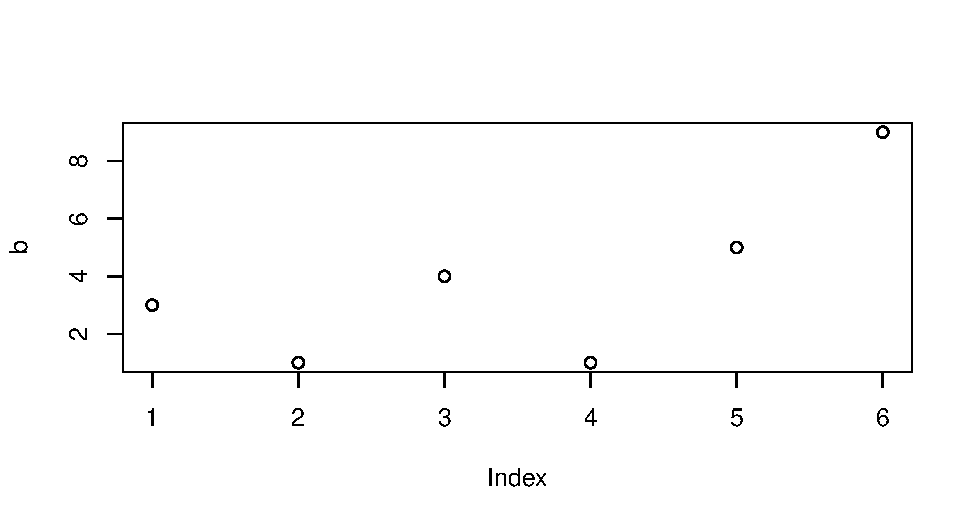
\includegraphics{R-anvisningar_files/figure-latex/unnamed-chunk-19-1} \end{center}

som ger en simpel graf, och

\begin{Shaded}
\begin{Highlighting}[]
\FunctionTok{sqrt}\NormalTok{(b)}
\end{Highlighting}
\end{Shaded}

\begin{verbatim}
## [1] 1.732051 1.000000 2.000000 1.000000 2.236068 3.000000
\end{verbatim}

som beräknar kvadratroten för varje element i vektorn.

\begin{exercise}[Summera vektorn]

Fyll i och kör följande rad för att beräkna summan av vektorn \texttt{new\_vector}

\begin{Shaded}
\begin{Highlighting}[]
\FunctionTok{sum}\NormalTok{(\_\_\_)}
\end{Highlighting}
\end{Shaded}

\end{exercise}

Vid konstruktionen av vektorn användes också en grundläggande funktion - funktionen \texttt{c} som tar en serie värden och skapar en sammanhängande vektor av värden.

Alla R-funktioner har en tillhörande hjälpfil som kan plockas fram genom att skriva frågetecken följt av funktionsnamnet, t.ex. \texttt{?sum}. Från hjälpfilen får man att \texttt{sum} tar numeriska vektorer som ingående värde och beräknar summan. Man kan styra funktionens beteende genom att sätta ett argument \texttt{na.rm} (vilket här styr hur funktionen hanterar saknade värden). Som illustration kan man titta på

\begin{Shaded}
\begin{Highlighting}[]
\NormalTok{b }\OtherTok{\textless{}{-}} \FunctionTok{c}\NormalTok{(}\DecValTok{3}\NormalTok{, }\DecValTok{1}\NormalTok{, }\DecValTok{4}\NormalTok{, }\DecValTok{1}\NormalTok{, }\DecValTok{5}\NormalTok{, }\DecValTok{9}\NormalTok{, }\ConstantTok{NA}\NormalTok{)  }\CommentTok{\# Lägger till ett saknat värde}
\FunctionTok{sum}\NormalTok{(b)                        }\CommentTok{\# na.rm = FALSE är grundinställning}
\end{Highlighting}
\end{Shaded}

\begin{verbatim}
## [1] NA
\end{verbatim}

\begin{Shaded}
\begin{Highlighting}[]
\FunctionTok{sum}\NormalTok{(b, }\AttributeTok{na.rm =} \ConstantTok{TRUE}\NormalTok{)          }\CommentTok{\# na.rm sätts till TRUE}
\end{Highlighting}
\end{Shaded}

\begin{verbatim}
## [1] 23
\end{verbatim}

Det första försöket \texttt{sum(b)} ger utfallet \texttt{NA}, men om man sätter \texttt{na.rm\ =\ TRUE} beräknas summan efter att det saknade värdet plockats bort. Notera också att skript kan kommenteras med \texttt{\#}.

\hypertarget{sekvenser-av-funktioner}{%
\section{Sekvenser av funktioner}\label{sekvenser-av-funktioner}}

Ofta vill man genomföra flera operationer på ett objekt. Man behöver då genomföra en sekvens av funktioner. Säg till exempel att man har värdena \[(-4, -2, -1, 1, 2, 4)\] och vill ta absolutvärde (vilket gör negativa tal till motsvarande positiva tal) och sedan summera.
Den typen av sekvenser kan genomföras på ett par olika sätt. Ett första sätt är att spara resultatet i varje steg och sedan använda utfallet i nästa steg:

\begin{Shaded}
\begin{Highlighting}[]
\NormalTok{c }\OtherTok{\textless{}{-}} \FunctionTok{c}\NormalTok{(}\SpecialCharTok{{-}}\DecValTok{4}\NormalTok{, }\SpecialCharTok{{-}}\DecValTok{2}\NormalTok{, }\SpecialCharTok{{-}}\DecValTok{1}\NormalTok{, }\DecValTok{1}\NormalTok{, }\DecValTok{2}\NormalTok{, }\DecValTok{4}\NormalTok{)}
\NormalTok{c\_absolute }\OtherTok{\textless{}{-}} \FunctionTok{abs}\NormalTok{(c)}
\FunctionTok{sum}\NormalTok{(c\_absolute)}
\end{Highlighting}
\end{Shaded}

\begin{verbatim}
## [1] 14
\end{verbatim}

Här skapas ett objekt \texttt{c} som innehåller en vektor där några tal är negativa. I nästa rad används \texttt{abs} för att skapa absolutvärden. Slutligen summeras absolutvärdena med \texttt{sum}.
Notera att det är möjligt att skapa ett objekt med namnet \texttt{c} trots att det redan är namnet på en funktion - R förstår ur sammanhanget om objektet eller funktionen ska användas.

\begin{exercise}[Kvadrat, summa och roten ur]

Fyll i och kör följande rader för att ta varje värde i \texttt{new\_vector} i kvadrat, \emph{sedan} summera, och sedan ta roten ur.

\begin{Shaded}
\begin{Highlighting}[]
\NormalTok{new\_vector\_squared }\OtherTok{\textless{}{-}}\NormalTok{ new\_vector}\SpecialCharTok{\^{}}\DecValTok{2} \CommentTok{\# Ta kvadraten av varje värde}
\NormalTok{new\_vector\_squared\_sum }\OtherTok{\textless{}{-}} \FunctionTok{sum}\NormalTok{(\_\_\_) }\CommentTok{\# Summera vektorn med kvadrater}
\FunctionTok{sqrt}\NormalTok{(\_\_\_)                          }\CommentTok{\# Ta kvadratroten ur summan}
\end{Highlighting}
\end{Shaded}

\end{exercise}

Ett alternativ är att skriva en senare funktion \emph{runt} en tidigare funktion. Det fungerar för att R utvärderar funktioner inifrån-ut. Med samma exempel som tidigare får man

\begin{Shaded}
\begin{Highlighting}[]
\FunctionTok{sum}\NormalTok{(}\FunctionTok{abs}\NormalTok{(}\FunctionTok{c}\NormalTok{(}\SpecialCharTok{{-}}\DecValTok{4}\NormalTok{, }\SpecialCharTok{{-}}\DecValTok{2}\NormalTok{, }\SpecialCharTok{{-}}\DecValTok{1}\NormalTok{, }\DecValTok{1}\NormalTok{, }\DecValTok{2}\NormalTok{, }\DecValTok{4}\NormalTok{)))}
\end{Highlighting}
\end{Shaded}

medan beräkningen i övningen blir

\begin{Shaded}
\begin{Highlighting}[]
\FunctionTok{sqrt}\NormalTok{(}\FunctionTok{sum}\NormalTok{(new\_vector}\SpecialCharTok{\^{}}\DecValTok{2}\NormalTok{))}
\end{Highlighting}
\end{Shaded}

Den här typen av skrivning kan spara plats men blir snabbt svårläst.

Ett sista alternativ är att använda en så kallad \emph{pipe} (namnet kommer från att en sekvens funktioner kallas en \emph{pipeline}). En pipe skrivs \texttt{\%\textgreater{}\%} och tar utfallet av en funktion till vänster och sänder till en funktion till höger. Språkligt kan pipen utläsas \emph{och sen}. Funktionen kan laddas genom att ladda paketet \texttt{tidyverse}. Med samma exempel som tidigare kan vi skriva

\begin{Shaded}
\begin{Highlighting}[]
\FunctionTok{library}\NormalTok{(tidyverse)}

\FunctionTok{c}\NormalTok{(}\SpecialCharTok{{-}}\DecValTok{4}\NormalTok{, }\SpecialCharTok{{-}}\DecValTok{2}\NormalTok{, }\SpecialCharTok{{-}}\DecValTok{1}\NormalTok{, }\DecValTok{1}\NormalTok{, }\DecValTok{2}\NormalTok{, }\DecValTok{4}\NormalTok{) }\SpecialCharTok{\%\textgreater{}\%}  \CommentTok{\# Skapa en datamängd och sen}
  \FunctionTok{abs}\NormalTok{() }\SpecialCharTok{\%\textgreater{}\%}                 \CommentTok{\# ta absolutvärden, och sen}
  \FunctionTok{sum}\NormalTok{()                     }\CommentTok{\# beräkna summan.}
\end{Highlighting}
\end{Shaded}

\begin{verbatim}
## [1] 14
\end{verbatim}

\begin{exercise}[Kvadrat, summa och rot med pipe]

Fyll i de saknade funktionerna och kör följande rader för att ta varje värde i \texttt{new\_vector} i kvadrat, \emph{sedan} summera, och sedan ta roten ur, denna gång genom att länka funktionerna med en pipe \texttt{\%\textgreater{}\%}.

\begin{Shaded}
\begin{Highlighting}[]
\NormalTok{new\_vector}\SpecialCharTok{\^{}}\DecValTok{2} \SpecialCharTok{\%\textgreater{}\%}        \CommentTok{\# Ta kvadraterna av new\_vector, och sen}
  \FunctionTok{\_\_\_}\NormalTok{() }\SpecialCharTok{\%\textgreater{}\%}             \CommentTok{\# beräkna summan, och sen}
  \FunctionTok{\_\_\_\_}\NormalTok{()                }\CommentTok{\# Ta kvadratroten (med sqrt())}
\end{Highlighting}
\end{Shaded}

\end{exercise}

\hypertarget{datainskrivning-och-dataimport-fruxe5n-web}{%
\section{Datainskrivning och dataimport från web}\label{datainskrivning-och-dataimport-fruxe5n-web}}

\hypertarget{inskrivning-av-data}{%
\subsection{Inskrivning av data}\label{inskrivning-av-data}}

Det första praktiska steget i en statistisk analys är att importera data. I R kan det göras genom att direkt skriva in sin data och spara som ett nytt objekt, men ett bättre och vanligare sätt är att importera sin data från en extern fil eller databas.

I ett tidigare exempel användes funktionen \texttt{c} för att skapa en vektor av data. Ofta ordnas flera vektorer i en tabell där varje kolumn är en vektor och varje rad en observation av någon enhet. En datatabell (en \texttt{data.frame} i R) skapas genom funktionen \texttt{data.frame()} följt av namngivna vektorer. Exempeldata kan skrivas in genom föjande.

\begin{Shaded}
\begin{Highlighting}[]
\NormalTok{dat }\OtherTok{\textless{}{-}} \FunctionTok{data.frame}\NormalTok{(}\AttributeTok{Vecka =} \FunctionTok{c}\NormalTok{(}\DecValTok{7}\NormalTok{,}\DecValTok{7}\NormalTok{,}\DecValTok{7}\NormalTok{,}\DecValTok{7}\NormalTok{,}\DecValTok{7}\NormalTok{,}\DecValTok{7}\NormalTok{,}\DecValTok{11}\NormalTok{,}\DecValTok{11}\NormalTok{,}\DecValTok{11}\NormalTok{,}\DecValTok{11}\NormalTok{,}\DecValTok{11}\NormalTok{,}\DecValTok{11}\NormalTok{),}
                  \AttributeTok{Behandling =} \FunctionTok{c}\NormalTok{(}\StringTok{"A"}\NormalTok{,}\StringTok{"A"}\NormalTok{,}\StringTok{"A"}\NormalTok{,}\StringTok{"B"}\NormalTok{,}\StringTok{"B"}\NormalTok{,}\StringTok{"B"}\NormalTok{,}\StringTok{"A"}\NormalTok{,}\StringTok{"A"}\NormalTok{,}\StringTok{"A"}\NormalTok{,}\StringTok{"B"}\NormalTok{,}\StringTok{"B"}\NormalTok{,}\StringTok{"B"}\NormalTok{),}
                  \AttributeTok{Vikt =} \FunctionTok{c}\NormalTok{(}\DecValTok{232}\NormalTok{,}\DecValTok{161}\NormalTok{,}\DecValTok{148}\NormalTok{,}\DecValTok{368}\NormalTok{,}\DecValTok{218}\NormalTok{,}\DecValTok{257}\NormalTok{,}\DecValTok{1633}\NormalTok{,}\DecValTok{2213}\NormalTok{,}\DecValTok{972}\NormalTok{,}\DecValTok{2560}\NormalTok{,}\DecValTok{2430}\NormalTok{,}\DecValTok{855}\NormalTok{),}
                  \AttributeTok{N =} \FunctionTok{c}\NormalTok{(}\FloatTok{2.63}\NormalTok{,}\FloatTok{2.90}\NormalTok{,}\FloatTok{2.99}\NormalTok{,}\FloatTok{3.54}\NormalTok{,}\FloatTok{3.30}\NormalTok{,}\FloatTok{2.85}\NormalTok{,}\FloatTok{1.53}\NormalTok{,}\FloatTok{1.90}\NormalTok{,}\ConstantTok{NA}\NormalTok{,}\FloatTok{2.58}\NormalTok{,}\ConstantTok{NA}\NormalTok{,}\ConstantTok{NA}\NormalTok{))}

\NormalTok{dat}
\end{Highlighting}
\end{Shaded}

\begin{verbatim}
##    Vecka Behandling Vikt    N
## 1      7          A  232 2.63
## 2      7          A  161 2.90
## 3      7          A  148 2.99
## 4      7          B  368 3.54
## 5      7          B  218 3.30
## 6      7          B  257 2.85
## 7     11          A 1633 1.53
## 8     11          A 2213 1.90
## 9     11          A  972   NA
## 10    11          B 2560 2.58
## 11    11          B 2430   NA
## 12    11          B  855   NA
\end{verbatim}

Radbrytningar och blanksteg är oviktiga i R, och används bara för läsbarhet här. Saknade värden skrivs in som \texttt{NA} för \emph{not available}. Notera att alla kolumner inte behöver vara av samma datatyp men att värden inom en kolumn måste vara det. Här är \emph{Behandling} text medan övriga kolumner är numeriska.

\begin{exercise}[Alea iacta est]

Kasta din tärning tio gånger och skriv in resultatet i en datatabell i R med hjälp av grundkoden nedan. Om du saknar en tärning, fråga lämplig person om du kan få en. Behåll tärningen, den behövs till nästa datorövning (och närhelst man står inför ett avgörande livsbeslut).

\begin{Shaded}
\begin{Highlighting}[]
\NormalTok{dat\_dice }\OtherTok{\textless{}{-}} \FunctionTok{data.frame}\NormalTok{(}\AttributeTok{Kast =} \FunctionTok{c}\NormalTok{(}\DecValTok{1}\NormalTok{,}\DecValTok{2}\NormalTok{,}\DecValTok{3}\NormalTok{,}\DecValTok{4}\NormalTok{,}\DecValTok{5}\NormalTok{,}\DecValTok{6}\NormalTok{,}\DecValTok{7}\NormalTok{,}\DecValTok{8}\NormalTok{,}\DecValTok{9}\NormalTok{,}\DecValTok{10}\NormalTok{),}
                       \AttributeTok{Utfall =} \FunctionTok{c}\NormalTok{(\_,\_,\_,\_,\_,\_,\_,\_,\_,\_))}
\NormalTok{dat\_dice}
\end{Highlighting}
\end{Shaded}

\end{exercise}

\hypertarget{import-fruxe5n-en-extern-fil}{%
\subsection{Import från en extern fil}\label{import-fruxe5n-en-extern-fil}}

Inskrivning av värden är ofta tidskrävande och kan lätt leda till misstag. Det är därför mycket vanligare att data läses in från en extern fil. Det finns en mängd funktioner för dataimport och det exakta valet av funktion beror på vilken typ av fil datan är sparad i. Ett vanligt filformat är .csv (\emph{comma separated values}). Här importerar vi en fil med data från Spotify.

\begin{Shaded}
\begin{Highlighting}[]
\NormalTok{dat }\OtherTok{\textless{}{-}} \FunctionTok{read\_csv}\NormalTok{(}\StringTok{"https://raw.githubusercontent.com/adamflr/ST0060/master/Data/Spotify\_data.csv"}\NormalTok{)}
\NormalTok{dat}
\end{Highlighting}
\end{Shaded}

\begin{verbatim}
## # A tibble: 76,622 x 24
##    artist_name album_name    track_number track_name album_type album_release_d~
##    <chr>       <chr>                <dbl> <chr>      <chr>      <chr>           
##  1 100 gecs    1000 gecs an~            1 money mac~ album      2020-07-10      
##  2 100 gecs    1000 gecs an~            2 ringtone ~ album      2020-07-10      
##  3 100 gecs    1000 gecs an~            3 745 stick~ album      2020-07-10      
##  4 100 gecs    1000 gecs an~            4 gec 2 Ü (~ album      2020-07-10      
##  5 100 gecs    1000 gecs an~            5 hand crus~ album      2020-07-10      
##  6 100 gecs    1000 gecs an~            6 800db clo~ album      2020-07-10      
##  7 100 gecs    1000 gecs an~            7 stupid ho~ album      2020-07-10      
##  8 100 gecs    1000 gecs an~            8 ringtone ~ album      2020-07-10      
##  9 100 gecs    1000 gecs an~            9 xXXi_wud_~ album      2020-07-10      
## 10 100 gecs    1000 gecs an~           10 745 stick~ album      2020-07-10      
## # ... with 76,612 more rows, and 18 more variables: album_release_year <dbl>,
## #   danceability <dbl>, energy <dbl>, key <dbl>, loudness <dbl>, mode <dbl>,
## #   speechiness <dbl>, acousticness <dbl>, instrumentalness <dbl>,
## #   liveness <dbl>, valence <dbl>, tempo <dbl>, time_signature <dbl>,
## #   explicit <lgl>, type <chr>, key_name <chr>, mode_name <chr>, key_mode <chr>
\end{verbatim}

Om importen fungerat kan man skriva ut tabellens översta rader genom att köra objektets namn.

För att snabbt se vilka artister datan täcker kan man köra

\begin{Shaded}
\begin{Highlighting}[]
\FunctionTok{unique}\NormalTok{(dat}\SpecialCharTok{$}\NormalTok{artist\_name)}
\end{Highlighting}
\end{Shaded}

där \texttt{unique} är en funktion som tar bort alla dubletter och \texttt{dat\$artist\_name} används för att plocka ut kolumnen \texttt{artist\_name} ur tabellen \texttt{dat}.

\hypertarget{transformera-en-tabell-med-select-filter-mutate-och-summarise}{%
\section{\texorpdfstring{Transformera en tabell med \texttt{select}, \texttt{filter}, \texttt{mutate} och \texttt{summarise}}{Transformera en tabell med select, filter, mutate och summarise}}\label{transformera-en-tabell-med-select-filter-mutate-och-summarise}}

\hypertarget{urval-med-select-och-filter}{%
\subsection{\texorpdfstring{Urval med \texttt{select} och \texttt{filter}}{Urval med select och filter}}\label{urval-med-select-och-filter}}

En vanlig operation på en tabell är att göra ett urval - antingen ett urval av rader (t.ex. en viss artist), vilket kallas \emph{filtrering} eller ett urval av variabler (t.ex. artist och albumnamn), vilket kallas \emph{selektion}.
Det finns flera olika sätt att göra ett urval i R.
Det traditionella sättet är att använda index inom hakparenteser (t.ex. \texttt{dat{[}4,\ 2{]}} för fjärde raden, andra kolumnen) eller dollartecken för specifika kolumner (t.ex. \texttt{dat\$artist\_name} för artistnamn).
Här fokuseras dock på hur det kan göras med funktionerna \texttt{filter} och \texttt{select} från paketet \texttt{tidyverse}.

För att filtrera på ett givet land kan använda pipe-funktionen från datan till en filter-funktion, t.ex.

\begin{Shaded}
\begin{Highlighting}[]
\NormalTok{dat }\SpecialCharTok{\%\textgreater{}\%}                          \CommentTok{\# Ta spotify{-}datan och sen}
  \FunctionTok{filter}\NormalTok{(artist\_name }\SpecialCharTok{==} \StringTok{"Robyn"}\NormalTok{) }\CommentTok{\# filtrera för en specifik artist}
\end{Highlighting}
\end{Shaded}

\begin{verbatim}
## # A tibble: 1,142 x 24
##    artist_name album_name track_number track_name    album_type album_release_d~
##    <chr>       <chr>             <dbl> <chr>         <chr>      <chr>           
##  1 Robyn       Honey                 1 Missing U     album      2018-10-26      
##  2 Robyn       Honey                 2 Human Being   album      2018-10-26      
##  3 Robyn       Honey                 3 Because It's~ album      2018-10-26      
##  4 Robyn       Honey                 4 Baby Forgive~ album      2018-10-26      
##  5 Robyn       Honey                 5 Send To Robi~ album      2018-10-26      
##  6 Robyn       Honey                 6 Honey         album      2018-10-26      
##  7 Robyn       Honey                 7 Between The ~ album      2018-10-26      
##  8 Robyn       Honey                 8 Beach2k20     album      2018-10-26      
##  9 Robyn       Honey                 9 Ever Again    album      2018-10-26      
## 10 Robyn       Honey                 1 Missing U     album      2018-10-26      
## # ... with 1,132 more rows, and 18 more variables: album_release_year <dbl>,
## #   danceability <dbl>, energy <dbl>, key <dbl>, loudness <dbl>, mode <dbl>,
## #   speechiness <dbl>, acousticness <dbl>, instrumentalness <dbl>,
## #   liveness <dbl>, valence <dbl>, tempo <dbl>, time_signature <dbl>,
## #   explicit <lgl>, type <chr>, key_name <chr>, mode_name <chr>, key_mode <chr>
\end{verbatim}

Inom filter-funktionen anges ett logisk villkor \texttt{country\ ==\ "Sweden"} och utfallet är de rader där villkoret är sant. Notera de dubbla likhetstecknen - de måste användas för ett logisk villkor eftersom enkelt likhetstecken används för att skapa objekt och sätta funktionsargument.

\begin{exercise}[Filtrera för artist]

Vad måste ändras i koden för att istället plocka ut rader där artisten är Esperanza Spalding? Hur många rader har det urvalet?

\begin{Shaded}
\begin{Highlighting}[]
\NormalTok{dat }\SpecialCharTok{\%\textgreater{}\%}                          \CommentTok{\# Ta spotify{-}datan och sen}
  \FunctionTok{filter}\NormalTok{(artist\_name }\SpecialCharTok{==} \StringTok{"Robyn"}\NormalTok{) }\CommentTok{\# filtrera för en specifik artist}
\end{Highlighting}
\end{Shaded}

\end{exercise}

Om man vill välja flera artister kan man använda funktionen \texttt{\%in\%} på ett liknande sätt.

\begin{Shaded}
\begin{Highlighting}[]
\NormalTok{dat }\SpecialCharTok{\%\textgreater{}\%} 
  \FunctionTok{filter}\NormalTok{(artist\_name }\SpecialCharTok{\%in\%} \FunctionTok{c}\NormalTok{(}\StringTok{"Robyn"}\NormalTok{, }\StringTok{"Esperanza Spalding"}\NormalTok{))}
\end{Highlighting}
\end{Shaded}

och om man vill ha mer än ett villkor kan man rada dem i filter-funktionen eller ha flera filter-steg:

\begin{Shaded}
\begin{Highlighting}[]
\NormalTok{dat }\SpecialCharTok{\%\textgreater{}\%} 
  \FunctionTok{filter}\NormalTok{(artist\_name }\SpecialCharTok{\%in\%} \FunctionTok{c}\NormalTok{(}\StringTok{"Robyn"}\NormalTok{, }\StringTok{"Esperanza Spalding"}\NormalTok{),}
\NormalTok{         key\_name }\SpecialCharTok{==} \StringTok{"D\#"}\NormalTok{)}
\end{Highlighting}
\end{Shaded}

alternativt

\begin{Shaded}
\begin{Highlighting}[]
\NormalTok{dat }\SpecialCharTok{\%\textgreater{}\%} 
  \FunctionTok{filter}\NormalTok{(artist\_name }\SpecialCharTok{\%in\%} \FunctionTok{c}\NormalTok{(}\StringTok{"Robyn"}\NormalTok{, }\StringTok{"Esperanza Spalding"}\NormalTok{)) }\SpecialCharTok{\%\textgreater{}\%} 
  \FunctionTok{filter}\NormalTok{(key\_name }\SpecialCharTok{==} \StringTok{"D\#"}\NormalTok{)}
\end{Highlighting}
\end{Shaded}

För att se fler eller färre rader kan man använda en pipe \texttt{\%\textgreater{}\%} till funktionen \texttt{print}. Följande skriver ut fem rader

\begin{Shaded}
\begin{Highlighting}[]
\NormalTok{dat }\SpecialCharTok{\%\textgreater{}\%} 
  \FunctionTok{filter}\NormalTok{(artist\_name }\SpecialCharTok{\%in\%} \FunctionTok{c}\NormalTok{(}\StringTok{"Robyn"}\NormalTok{, }\StringTok{"Esperanza Spalding"}\NormalTok{)) }\SpecialCharTok{\%\textgreater{}\%} 
  \FunctionTok{filter}\NormalTok{(key\_name }\SpecialCharTok{==} \StringTok{"D\#"}\NormalTok{) }\SpecialCharTok{\%\textgreater{}\%} 
  \FunctionTok{print}\NormalTok{(}\AttributeTok{n =} \DecValTok{5}\NormalTok{)}
\end{Highlighting}
\end{Shaded}

\begin{verbatim}
## # A tibble: 21 x 24
##   artist_name     album_name track_number track_name album_type album_release_d~
##   <chr>           <chr>             <dbl> <chr>      <chr>      <chr>           
## 1 Esperanza Spal~ SONGWRIGH~            7 Formwela 7 album      2021-09-24      
## 2 Esperanza Spal~ 12 Little~            2 To Tide U~ album      2019-05-10      
## 3 Esperanza Spal~ 12 Little~            3 'Til the ~ album      2019-05-10      
## 4 Esperanza Spal~ Emily’s D~            7 Ebony And~ album      2016-01-01      
## 5 Esperanza Spal~ Emily’s D~            7 Ebony And~ album      2016-01-01      
## # ... with 16 more rows, and 18 more variables: album_release_year <dbl>,
## #   danceability <dbl>, energy <dbl>, key <dbl>, loudness <dbl>, mode <dbl>,
## #   speechiness <dbl>, acousticness <dbl>, instrumentalness <dbl>,
## #   liveness <dbl>, valence <dbl>, tempo <dbl>, time_signature <dbl>,
## #   explicit <lgl>, type <chr>, key_name <chr>, mode_name <chr>, key_mode <chr>
\end{verbatim}

Om man istället vill göra ett urval av kolumner kan man använda \texttt{select}. Som argument anges de kolumner man vill välja, t.ex.

\begin{Shaded}
\begin{Highlighting}[]
\NormalTok{dat }\SpecialCharTok{\%\textgreater{}\%} 
  \FunctionTok{select}\NormalTok{(artist\_name, album\_name)}
\end{Highlighting}
\end{Shaded}

\begin{verbatim}
## # A tibble: 76,622 x 2
##    artist_name album_name                     
##    <chr>       <chr>                          
##  1 100 gecs    1000 gecs and The Tree of Clues
##  2 100 gecs    1000 gecs and The Tree of Clues
##  3 100 gecs    1000 gecs and The Tree of Clues
##  4 100 gecs    1000 gecs and The Tree of Clues
##  5 100 gecs    1000 gecs and The Tree of Clues
##  6 100 gecs    1000 gecs and The Tree of Clues
##  7 100 gecs    1000 gecs and The Tree of Clues
##  8 100 gecs    1000 gecs and The Tree of Clues
##  9 100 gecs    1000 gecs and The Tree of Clues
## 10 100 gecs    1000 gecs and The Tree of Clues
## # ... with 76,612 more rows
\end{verbatim}

Som avslutning ges ett lite mer komplicerat exempel på ett urval av artist, år och spår för spår med ett tempo över 180 bpm släppta under 2015.

\begin{Shaded}
\begin{Highlighting}[]
\NormalTok{dat }\SpecialCharTok{\%\textgreater{}\%}                                               \CommentTok{\# Ta datan och sen}
  \FunctionTok{filter}\NormalTok{(album\_release\_year }\SpecialCharTok{==} \DecValTok{2015}\NormalTok{,                  }\CommentTok{\# filtrera för rader där år är 2015, och }
\NormalTok{         tempo }\SpecialCharTok{\textgreater{}} \DecValTok{180}\NormalTok{) }\SpecialCharTok{\%\textgreater{}\%}                             \CommentTok{\# tempot över 160, och sen}
  \FunctionTok{select}\NormalTok{(artist\_name, album\_release\_year, track\_name) }\CommentTok{\# selektera på artist, år och spår}
\end{Highlighting}
\end{Shaded}

\begin{verbatim}
## # A tibble: 122 x 3
##    artist_name            album_release_year track_name                         
##    <chr>                               <dbl> <chr>                              
##  1 A Sunny Day In Glasgow               2015 The Strange Presents of Idols (Mer~
##  2 A$AP Rocky                           2015 Lord Pretty Flacko Jodye 2 (LPFJ2) 
##  3 A$AP Rocky                           2015 Lord Pretty Flacko Jodye 2 (LPFJ2) 
##  4 Anderson .Paak                       2015 Off the Ground                     
##  5 Björk                                2015 Notget - Live                      
##  6 Björk                                2015 Notget                             
##  7 Björk                                2015 Notget                             
##  8 Björk                                2015 Notget                             
##  9 Blood Orange                         2015 Sandra’s Smile                     
## 10 Burna Boy                            2015 Soke                               
## # ... with 112 more rows
\end{verbatim}

\begin{exercise}[Snabba spår]
Funktionen \texttt{arrange} sorterar data efter en angiven kolumn. Följande stycke ger oss Björks snabbaste spår.

\begin{Shaded}
\begin{Highlighting}[]
\NormalTok{dat }\SpecialCharTok{\%\textgreater{}\%}                                                   \CommentTok{\# Ta datan, och sen}
  \FunctionTok{filter}\NormalTok{(artist\_name }\SpecialCharTok{==} \StringTok{"Björk"}\NormalTok{) }\SpecialCharTok{\%\textgreater{}\%}                      \CommentTok{\# filtrera för rader där artist är Björk, och sen}
  \FunctionTok{select}\NormalTok{(artist\_name, album\_name, track\_name, tempo) }\SpecialCharTok{\%\textgreater{}\%}  \CommentTok{\# välj kolumner med artist, album, spår och tempo, och sen}
  \FunctionTok{arrange}\NormalTok{(}\SpecialCharTok{{-}}\NormalTok{tempo)                                         }\CommentTok{\# ordna efter tempo (minus för fallande ordning)}
\end{Highlighting}
\end{Shaded}

Gör lämpliga ändringar för att hitta Kate Bushs snabbaste spår. Gör ytterligare ändringar för att hitta Daft Punks långsammaste spår.
\end{exercise}

\hypertarget{uxe4ndra-och-skapa-nya-kolumner-med-mutate}{%
\subsection{\texorpdfstring{Ändra och skapa nya kolumner med \texttt{mutate}}{Ändra och skapa nya kolumner med mutate}}\label{uxe4ndra-och-skapa-nya-kolumner-med-mutate}}

Variabler kan omräknas och nya variabler kan skapas med \texttt{mutate}-funktionen. I spotify-datan finns tempo som slag per minut. Om man vill ha slag per sekund kan man skapa en nya kolumn och beräkna den som tempo delat på 60.

\begin{Shaded}
\begin{Highlighting}[]
\NormalTok{dat }\OtherTok{\textless{}{-}}\NormalTok{ dat }\SpecialCharTok{\%\textgreater{}\%} 
  \FunctionTok{mutate}\NormalTok{(}\AttributeTok{beats\_per\_second =}\NormalTok{ tempo }\SpecialCharTok{/} \DecValTok{60}\NormalTok{)}
\end{Highlighting}
\end{Shaded}

Den inledande delen med \texttt{dat\ \textless{}-} gör så att utfallet av beräkningen sparas i objektet \texttt{dat}.
Vi kan skriva ut objektet och se resultatet av beräkningen:

\begin{Shaded}
\begin{Highlighting}[]
\NormalTok{dat }\SpecialCharTok{\%\textgreater{}\%} \FunctionTok{select}\NormalTok{(tempo, beats\_per\_second)}
\end{Highlighting}
\end{Shaded}

\begin{verbatim}
## # A tibble: 76,622 x 2
##    tempo beats_per_second
##    <dbl>            <dbl>
##  1  132.             2.20
##  2  107.             1.78
##  3  128.             2.14
##  4  113.             1.89
##  5  174.             2.89
##  6  142.             2.36
##  7  166.             2.77
##  8  125.             2.08
##  9  170.             2.83
## 10  150.             2.50
## # ... with 76,612 more rows
\end{verbatim}

\begin{exercise}[Glädje per dansbarhet]
Följande stycke beräknar kvoten av kolumnerna valence och danceability i en ny kolumn `valence\_to\_danceability.

\begin{Shaded}
\begin{Highlighting}[]
\NormalTok{dat }\SpecialCharTok{\%\textgreater{}\%}                                                        \CommentTok{\# Ta datan, och sen}
  \FunctionTok{mutate}\NormalTok{(}\AttributeTok{valence\_to\_danceability =}\NormalTok{ valence }\SpecialCharTok{/}\NormalTok{ danceability) }\SpecialCharTok{\%\textgreater{}\%} \CommentTok{\# beräkna valence delat på danceability, och sen}
  \FunctionTok{select}\NormalTok{(valence, danceability, valence\_to\_danceability)       }\CommentTok{\# välj relevanta kolumner.}
\end{Highlighting}
\end{Shaded}

Gör lämpliga ändringar för att multiplicera \texttt{tempo} och \texttt{time\ signature}.
\end{exercise}

\hypertarget{summera-kolumner-med-group_by-och-summarise}{%
\subsection{\texorpdfstring{Summera kolumner med \texttt{group\_by} och \texttt{summarise}}{Summera kolumner med group\_by och summarise}}\label{summera-kolumner-med-group_by-och-summarise}}

För att presentera insamlad data på ett tolkningsbart sätt används sammanfattande mått såsom summor, medelvärden, medianer och standardavvikelser.
Den typen av beräkningar kan göras som ett nytt steg i en pipe med hjälp av funktionen \texttt{summarise}. Om man kombinerar \texttt{summarise} med funktionen \texttt{group\_by} kan man dessutom summera efter en indelning given av en annan variabel. En beräkning av genomsnittligt tempo per år kan till exempel ges av

\begin{Shaded}
\begin{Highlighting}[]
\NormalTok{dat }\SpecialCharTok{\%\textgreater{}\%}                                       \CommentTok{\# Ta datan, och sen}
  \FunctionTok{group\_by}\NormalTok{(album\_release\_year) }\SpecialCharTok{\%\textgreater{}\%}            \CommentTok{\# gruppera efter år, och sen}
  \FunctionTok{summarise}\NormalTok{(}\AttributeTok{Medeltempo =} \FunctionTok{mean}\NormalTok{(tempo))         }\CommentTok{\# beräkna medelvärde av tempo}
\end{Highlighting}
\end{Shaded}

\begin{verbatim}
## # A tibble: 63 x 2
##    album_release_year Medeltempo
##                 <dbl>      <dbl>
##  1               1960      103. 
##  2               1961      104. 
##  3               1962      121. 
##  4               1963      116. 
##  5               1964      122. 
##  6               1965      114. 
##  7               1966      121. 
##  8               1967      118. 
##  9               1968       95.0
## 10               1969      116. 
## # ... with 53 more rows
\end{verbatim}

I det sista steget skapas en variabel \emph{Medeltempo} som ges av medelvärde av den ursprungliga variabeln \emph{tempo}. Här använder vi också funktionen \texttt{mean} för att beräkna medelvärdet.

Om man vill summera flera variabler kan man ange flera beräkning inom \texttt{summarise}, t.ex.

\begin{Shaded}
\begin{Highlighting}[]
\NormalTok{dat }\SpecialCharTok{\%\textgreater{}\%}                                   \CommentTok{\# Ta datan, och sen}
  \FunctionTok{group\_by}\NormalTok{(album\_release\_year) }\SpecialCharTok{\%\textgreater{}\%}        \CommentTok{\# gruppera efter år, och sen}
  \FunctionTok{summarise}\NormalTok{(}\AttributeTok{Medeltempo =} \FunctionTok{mean}\NormalTok{(tempo),     }\CommentTok{\# beräkna medelvärde av tempo}
            \AttributeTok{Medelvalence =} \FunctionTok{mean}\NormalTok{(valence), }\CommentTok{\# beräkna medelvärde av valence}
\NormalTok{            antal\_spår }\OtherTok{=} \FunctionTok{n}\NormalTok{()) }\SpecialCharTok{\%\textgreater{}\%}         \CommentTok{\# beräkna antalet spår, och sen}
  \FunctionTok{arrange}\NormalTok{(}\SpecialCharTok{{-}}\NormalTok{Medelvalence)                  }\CommentTok{\# ordna efter medelvalence i sjunkande ordning}
\end{Highlighting}
\end{Shaded}

\begin{verbatim}
## # A tibble: 63 x 4
##    album_release_year Medeltempo Medelvalence antal_spår
##                 <dbl>      <dbl>        <dbl>      <int>
##  1               1960      103.         0.816         29
##  2               1961      104.         0.752         12
##  3               1968       95.0        0.738         21
##  4               1981      123.         0.671         17
##  5               1965      114.         0.642        147
##  6               1972      118.         0.641         64
##  7               1976      123.         0.626         65
##  8               1982      114.         0.624         50
##  9               1975      123.         0.622         84
## 10               1962      121.         0.613         13
## # ... with 53 more rows
\end{verbatim}

\begin{exercise}[Gladast artist]

Vad ska ändras i stycket ovan för att beräkna medelvalence per artist istället för per år?

Vad måste ändras i stycket nedan för att se vilka artister som påverkar värdet för 1960?

\begin{Shaded}
\begin{Highlighting}[]
\NormalTok{dat }\SpecialCharTok{\%\textgreater{}\%} 
  \FunctionTok{filter}\NormalTok{(album\_release\_year }\SpecialCharTok{==} \DecValTok{1976}\NormalTok{) }\SpecialCharTok{\%\textgreater{}\%} 
  \FunctionTok{count}\NormalTok{(artist\_name, album\_name, album\_release\_year)}
\end{Highlighting}
\end{Shaded}

\end{exercise}

\hypertarget{grafer-med-ggplot2}{%
\section{\texorpdfstring{Grafer med \texttt{ggplot2}}{Grafer med ggplot2}}\label{grafer-med-ggplot2}}

Vi kan nu börja titta på grafer. Eftersom datan är ganska stor och grafer lätt blir oöversiktliga, börjar vi med att skapa en lite mindre datamängd.

\begin{Shaded}
\begin{Highlighting}[]
\NormalTok{dat\_small }\OtherTok{\textless{}{-}}\NormalTok{ dat }\SpecialCharTok{\%\textgreater{}\%} 
  \FunctionTok{filter}\NormalTok{(artist\_name }\SpecialCharTok{==} \StringTok{"Robyn"}\NormalTok{, album\_type }\SpecialCharTok{==} \StringTok{"album"}\NormalTok{)}
\end{Highlighting}
\end{Shaded}

\begin{exercise}[Valfritt artistbyte]
Om du vill titta data på något annan artist, gör lämplig ändring i stycket ovan. Kom ihåg att man skriva ut artister i datan med \texttt{unique(dat\$artist\_name)}.
\end{exercise}

R har en mängd grundläggande funktioner för grafer. Ett enkelt spridningsdiagram kan till exempel skapas med

\begin{Shaded}
\begin{Highlighting}[]
\FunctionTok{plot}\NormalTok{(}\AttributeTok{x =}\NormalTok{ dat\_small}\SpecialCharTok{$}\NormalTok{tempo, }\AttributeTok{y =}\NormalTok{ dat\_small}\SpecialCharTok{$}\NormalTok{danceability)}
\end{Highlighting}
\end{Shaded}

\begin{center}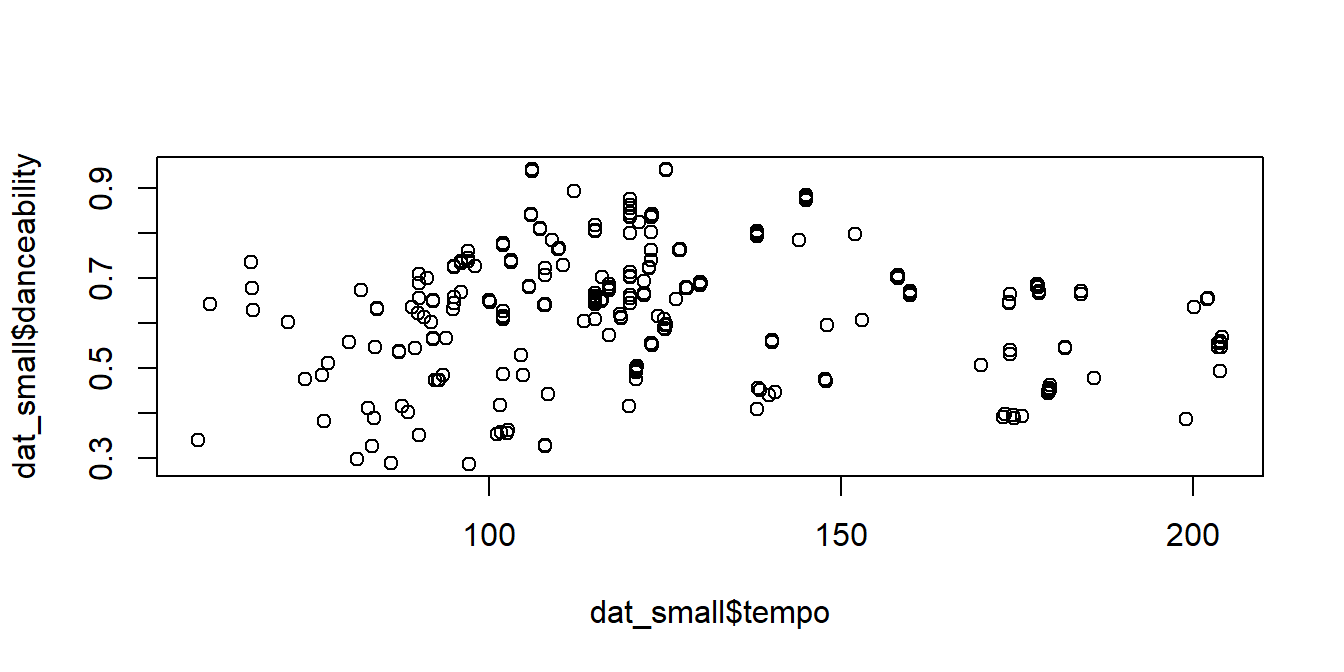
\includegraphics{R-anvisningar_files/figure-latex/unnamed-chunk-49-1} \end{center}

Tecknet \texttt{\$} används här för att välja en kolumn i en tabell.

För mer avancerade grafer används dock ofta funktioner ur Rs paketbibliotek. Här illustreras det mest populära - \texttt{ggplot2}. I \texttt{ggplot2} byggs grafer upp med tre grundläggande byggstenar:

\begin{itemize}
\tightlist
\item
  \emph{data}, informationen man vill visualisera,
\item
  \emph{aestethics}, en koppling mellan data och visuella element såsom grafens axlar, objekts storlek och färg,
\item
  \emph{geometries}, de geometriska former som visas i grafen.
\end{itemize}

En graf skrivs med en startfunktion \texttt{ggplot} som anger namnet på datan och grafens \emph{aestethics}, och därefter sätts geometriska element genom funktioner som börjar med \texttt{geom\_}. Ett spridningsdiagram kan t.ex. skapas med \texttt{geom\_point}.

\begin{Shaded}
\begin{Highlighting}[]
\FunctionTok{ggplot}\NormalTok{(dat\_small, }\FunctionTok{aes}\NormalTok{(}\AttributeTok{x =}\NormalTok{ tempo, }\AttributeTok{y =}\NormalTok{ danceability)) }\SpecialCharTok{+}
  \FunctionTok{geom\_point}\NormalTok{()}
\end{Highlighting}
\end{Shaded}

\begin{center}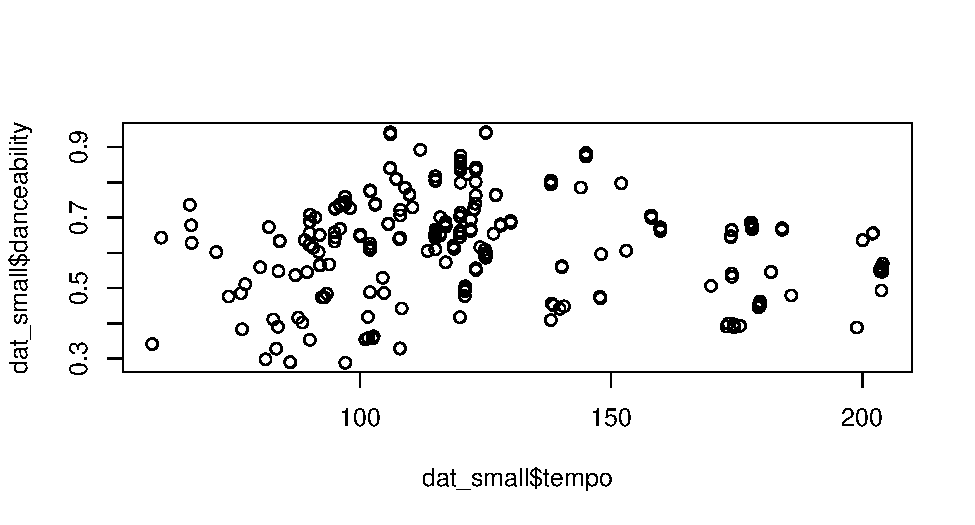
\includegraphics{R-anvisningar_files/figure-latex/unnamed-chunk-50-1} \end{center}

Grafen kan byggas ut genom att sätta \emph{aestethics} för färg och storlek. Man kan också dela en graf i småfönster med \texttt{facet\_wrap} och styra grafens utseende genom att sätta ett tema såsom \texttt{theme\_bw}.

\begin{Shaded}
\begin{Highlighting}[]
\FunctionTok{ggplot}\NormalTok{(dat\_small, }\FunctionTok{aes}\NormalTok{(}\AttributeTok{x =}\NormalTok{ tempo, }\AttributeTok{y =}\NormalTok{ danceability, }\AttributeTok{color =}\NormalTok{ mode\_name)) }\SpecialCharTok{+}
  \FunctionTok{geom\_point}\NormalTok{() }\SpecialCharTok{+}
  \FunctionTok{facet\_wrap}\NormalTok{(}\SpecialCharTok{\textasciitilde{}}\NormalTok{ album\_name)}
\end{Highlighting}
\end{Shaded}

\begin{center}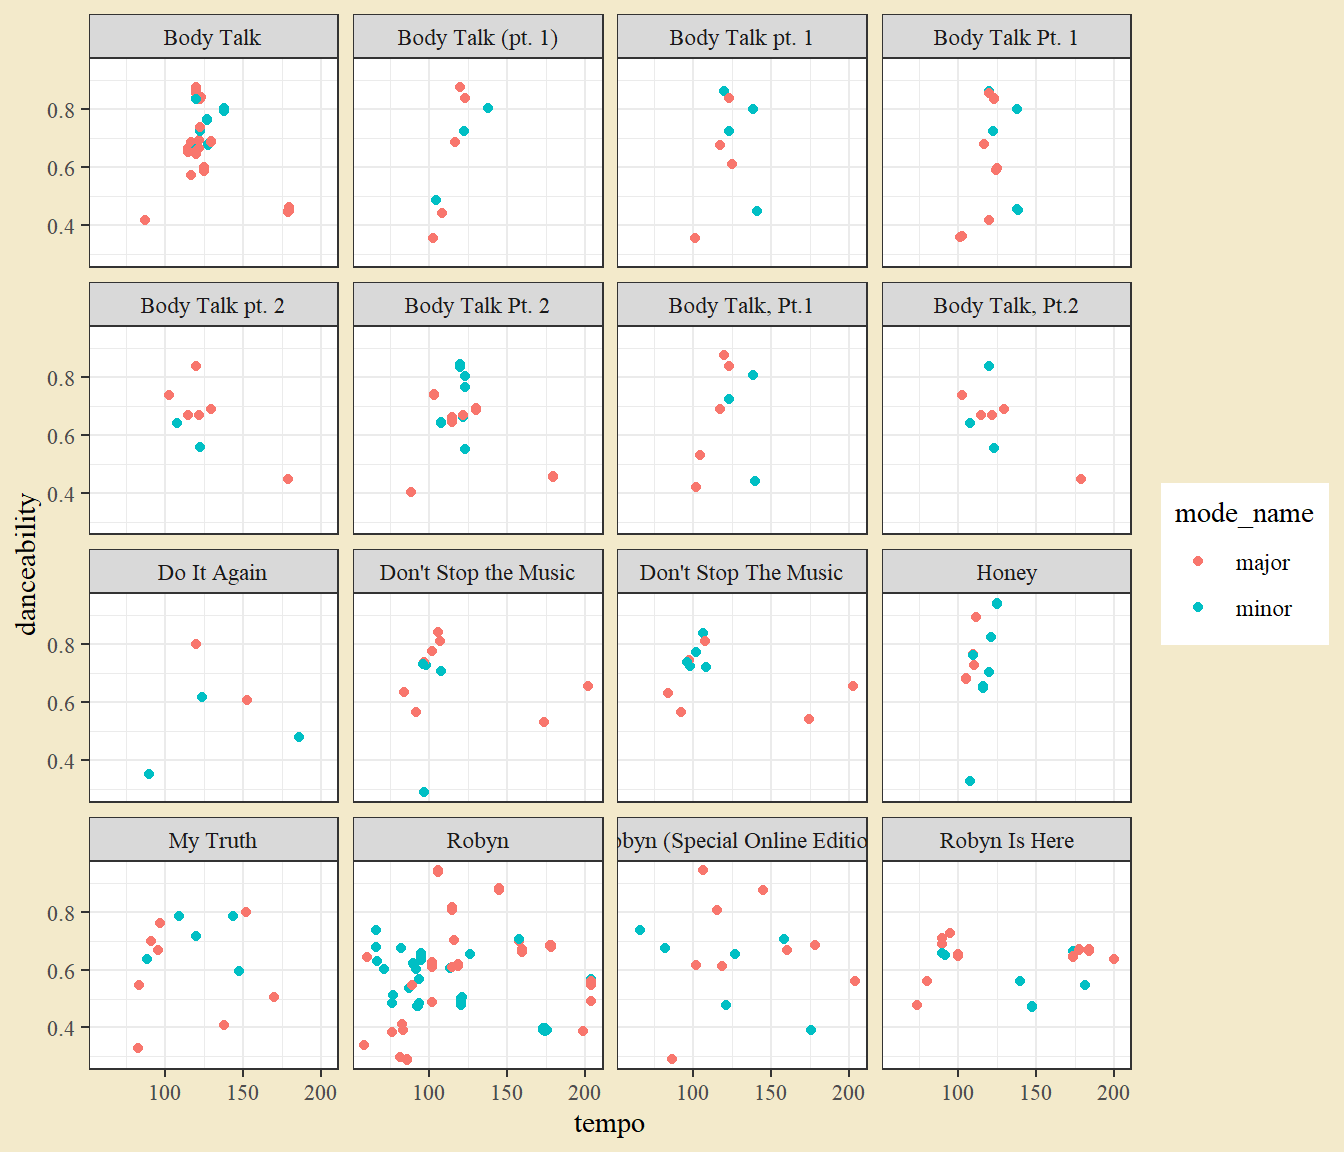
\includegraphics{R-anvisningar_files/figure-latex/unnamed-chunk-51-1} \end{center}

\begin{exercise}[Dur och moll]
Vad ska ändras i stycket nedan för att skapa en graf med dur/moll (\texttt{mode\_name}) på x-axeln, valens (\texttt{valence}) på y-axeln och skilda småfönster för olika år (\texttt{album\_release\_year})?

\begin{Shaded}
\begin{Highlighting}[]
\FunctionTok{ggplot}\NormalTok{(dat\_small, }\FunctionTok{aes}\NormalTok{(}\AttributeTok{x =}\NormalTok{ mode\_name, }\AttributeTok{y =}\NormalTok{ valence, }\AttributeTok{color =}\NormalTok{ album\_name)) }\SpecialCharTok{+}
  \FunctionTok{geom\_point}\NormalTok{() }\SpecialCharTok{+}
  \FunctionTok{facet\_wrap}\NormalTok{(}\SpecialCharTok{\textasciitilde{}}\NormalTok{ album\_release\_year)}
\end{Highlighting}
\end{Shaded}

Har spår i dur (\emph{major}) högre valens?
\end{exercise}

Andra graftyper kan skapas med andra \texttt{geom\_}-funktioner. För ett linjediagram används \texttt{geom\_line}. De observationer som ska ge en specifik linje anges med \texttt{group} i \texttt{aes}-funktionen. Låt oss beräkna medeldansbarhet över tid, uppdelat efter markeringen för \emph{explicit} (alltså om spåret är barnvänligt eller inte).

\begin{Shaded}
\begin{Highlighting}[]
\NormalTok{dat\_mean\_over\_time }\OtherTok{\textless{}{-}}\NormalTok{ dat }\SpecialCharTok{\%\textgreater{}\%} 
  \FunctionTok{group\_by}\NormalTok{(album\_release\_year, explicit) }\SpecialCharTok{\%\textgreater{}\%} 
  \FunctionTok{summarise}\NormalTok{(}\AttributeTok{Mean\_danceability =} \FunctionTok{mean}\NormalTok{(danceability))}

\FunctionTok{ggplot}\NormalTok{(dat\_mean\_over\_time, }\FunctionTok{aes}\NormalTok{(}\AttributeTok{x =}\NormalTok{ album\_release\_year, }\AttributeTok{y =}\NormalTok{ Mean\_danceability, }\AttributeTok{color =}\NormalTok{ explicit)) }\SpecialCharTok{+}
  \FunctionTok{geom\_line}\NormalTok{()}
\end{Highlighting}
\end{Shaded}

\begin{center}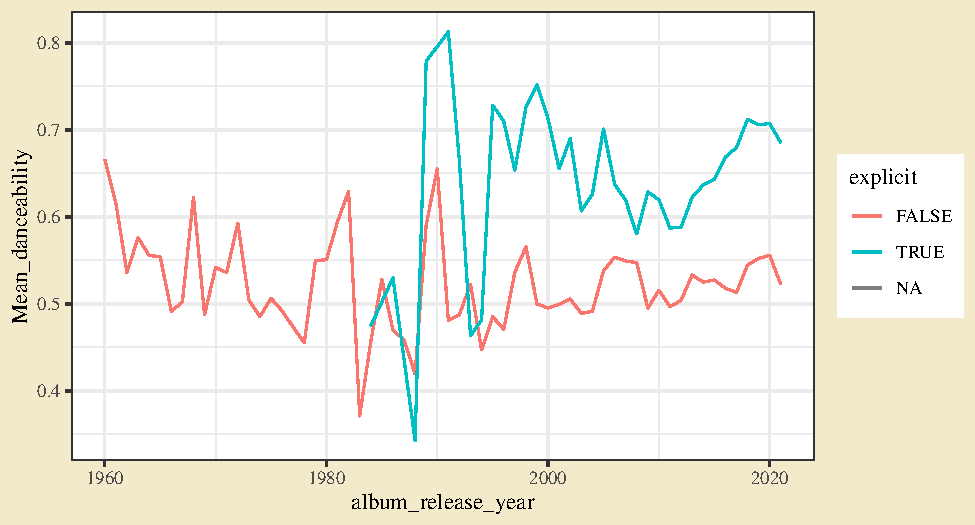
\includegraphics{R-anvisningar_files/figure-latex/unnamed-chunk-53-1} \end{center}

Här ger färgen uppdelningen i explicit och icke-explicit (\texttt{TRUE} för explicit). Det finns också spår som saknat värde för explicit och därför blir \texttt{NA} här. Kan vi utifrån grafen säga att barnvänlig musik är mer eller mindre dansbar än icke-barnvänlig?

\begin{exercise}[Explicit glädje]
Vad ska ändras i stycket ovan för att för en graf över medelvalens (\texttt{valence}) istället för dansbarhet? Är barnvänlig musik gladare eller ledsnare är icke-barnvänlig?
\end{exercise}

Stapeldiagram ges av \texttt{geom\_col} (\texttt{col} för \emph{column}). Man kan också använda \texttt{geom\_bar} om man bara vill räkna antal rader per någon kategori. Följande beräknar valens per artist, ordnar efter valens, väljer ut de tjugo högsta, och plottar i ett (liggande) stapeldiagram.

\begin{Shaded}
\begin{Highlighting}[]
\NormalTok{dat }\SpecialCharTok{\%\textgreater{}\%}                                                                  \CommentTok{\# Ta datan, och sen}
  \FunctionTok{group\_by}\NormalTok{(artist\_name) }\SpecialCharTok{\%\textgreater{}\%}                                              \CommentTok{\# gruppera efter artist, och sen}
  \FunctionTok{summarise}\NormalTok{(}\AttributeTok{Mean\_valence =} \FunctionTok{mean}\NormalTok{(valence)) }\SpecialCharTok{\%\textgreater{}\%}                            \CommentTok{\# ta medelvärdet av valence, och sen}
  \FunctionTok{arrange}\NormalTok{(}\SpecialCharTok{{-}}\NormalTok{Mean\_valence) }\SpecialCharTok{\%\textgreater{}\%}                                             \CommentTok{\# ordna efter medelvalens (minustecken för sjunkande ordning), och sen}
  \FunctionTok{slice}\NormalTok{(}\DecValTok{1}\SpecialCharTok{:}\DecValTok{20}\NormalTok{) }\SpecialCharTok{\%\textgreater{}\%}                                                        \CommentTok{\# ta ut de tjugo första raderna}
  \FunctionTok{ggplot}\NormalTok{(}\FunctionTok{aes}\NormalTok{(}\AttributeTok{x =}\NormalTok{ Mean\_valence, }\AttributeTok{y =}\NormalTok{ artist\_name, }\AttributeTok{fill =}\NormalTok{ Mean\_valence)) }\SpecialCharTok{+}  \CommentTok{\# starta en ggplot där x{-}axeln ges av valens och y{-}axeln av artist, och sen}
  \FunctionTok{geom\_col}\NormalTok{(}\AttributeTok{color =} \StringTok{"black"}\NormalTok{)                                              }\CommentTok{\# skapa en geometri av kolumner}
\end{Highlighting}
\end{Shaded}

\begin{center}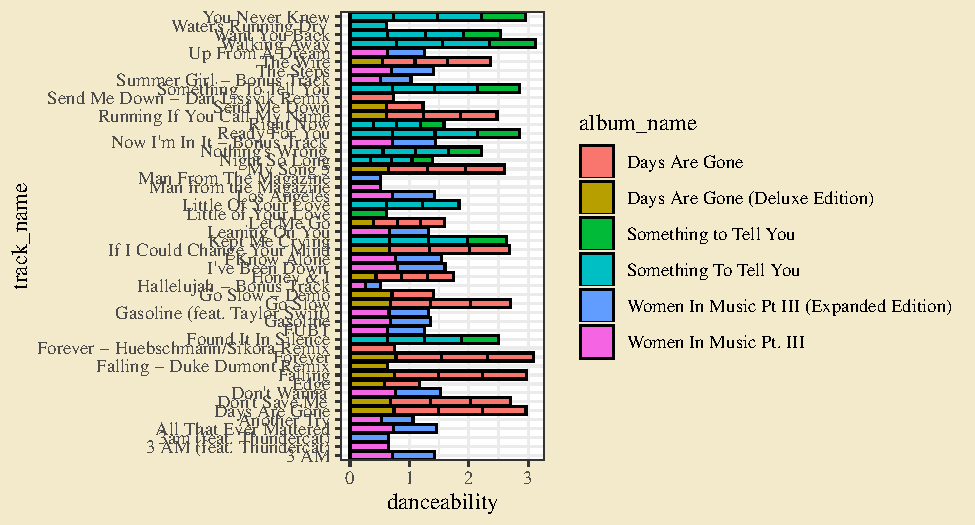
\includegraphics{R-anvisningar_files/figure-latex/unnamed-chunk-54-1} \end{center}

Argumentet \texttt{fill} styr färgen för ytor (här staplarnas ytor) medan \texttt{color} i \texttt{geom\_col()} styr kanten runt varje stapel.

Man kan styra grafiken i en \texttt{ggplot} genom funktionen \texttt{theme()}. Det är ett ganska komplicerat ämne, men låt oss titta på några grunder. Vi börjar med att skapa en enkel graf: en boxplot över dansbarhet per album för bandet \emph{Beach House} (som spelade på Malmöfestivalen 2009).

\begin{Shaded}
\begin{Highlighting}[]
\NormalTok{dat\_small }\OtherTok{\textless{}{-}}\NormalTok{ dat }\SpecialCharTok{\%\textgreater{}\%} \FunctionTok{filter}\NormalTok{(artist\_name }\SpecialCharTok{==} \StringTok{"Beach House"}\NormalTok{, album\_type }\SpecialCharTok{==} \StringTok{"album"}\NormalTok{)}

\FunctionTok{ggplot}\NormalTok{(dat\_small, }\FunctionTok{aes}\NormalTok{(danceability, album\_name)) }\SpecialCharTok{+}
  \FunctionTok{geom\_boxplot}\NormalTok{()}
\end{Highlighting}
\end{Shaded}

\begin{center}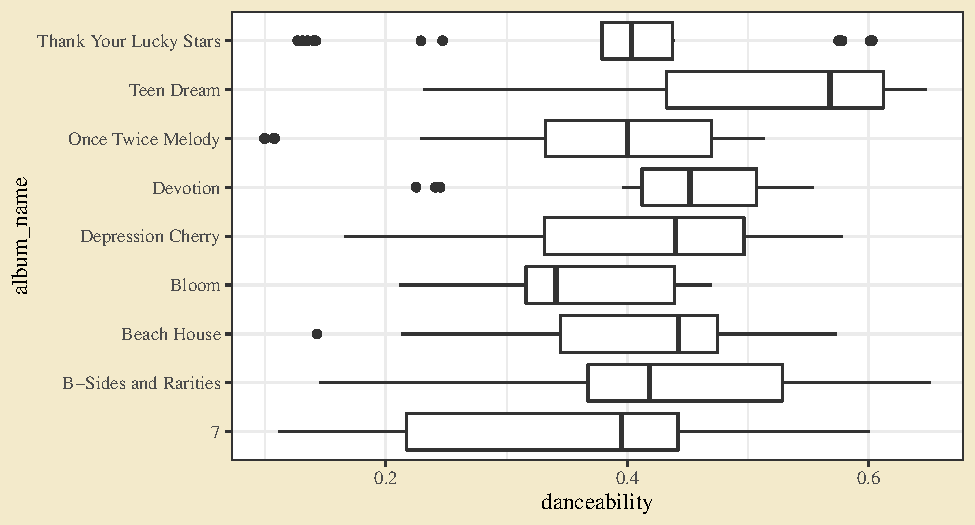
\includegraphics{R-anvisningar_files/figure-latex/unnamed-chunk-55-1} \end{center}

Vi kan ändra utseendet på grafen genom argument inom geometrier och med funktionen \texttt{theme()}. I \texttt{theme()} sätter man de specifika egenskaper man vill ändra genom att tillskriva dem ett \emph{element}. Valet av element beror på typen av grafiskt objekt - text sätts t.ex. med \texttt{element\_text()} och ytor med \texttt{element\_rect()} (för \emph{rectangle}). Vi ger ett exempel med ändrad bakgrund, rutmönster, och teckenstorlek.

\begin{Shaded}
\begin{Highlighting}[]
\FunctionTok{ggplot}\NormalTok{(dat\_small, }\FunctionTok{aes}\NormalTok{(danceability, album\_name)) }\SpecialCharTok{+}
  \FunctionTok{geom\_boxplot}\NormalTok{(}\AttributeTok{fill =} \StringTok{"lightblue"}\NormalTok{) }\SpecialCharTok{+}
  \FunctionTok{theme}\NormalTok{(}\AttributeTok{panel.background =} \FunctionTok{element\_rect}\NormalTok{(}\AttributeTok{fill =} \StringTok{"red3"}\NormalTok{), }
        \AttributeTok{text =} \FunctionTok{element\_text}\NormalTok{(}\AttributeTok{size =} \DecValTok{15}\NormalTok{, }\AttributeTok{color =} \StringTok{"white"}\NormalTok{, }\AttributeTok{family =} \StringTok{"serif"}\NormalTok{),}
        \AttributeTok{axis.text =} \FunctionTok{element\_text}\NormalTok{(}\AttributeTok{color =} \StringTok{"white"}\NormalTok{),}
        \AttributeTok{plot.background =} \FunctionTok{element\_rect}\NormalTok{(}\AttributeTok{fill =} \StringTok{"grey30"}\NormalTok{, }\AttributeTok{color =} \StringTok{"black"}\NormalTok{),}
        \AttributeTok{panel.grid.major.y =} \FunctionTok{element\_blank}\NormalTok{())}
\end{Highlighting}
\end{Shaded}

\begin{center}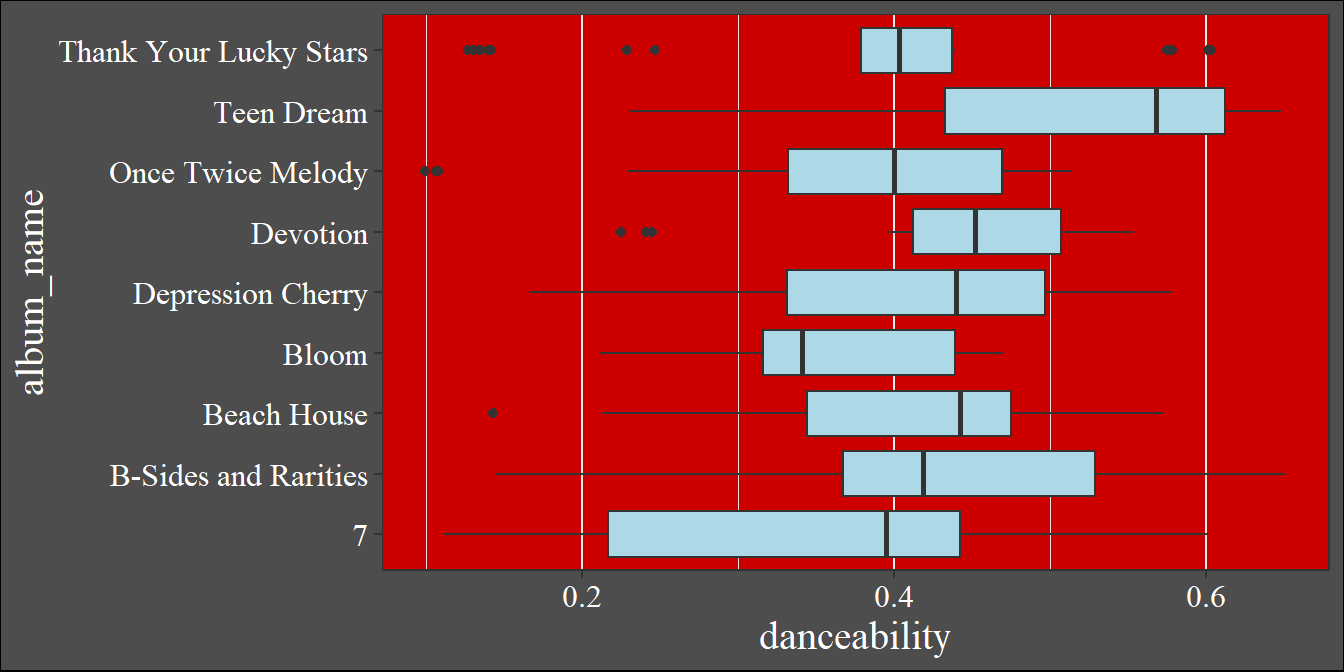
\includegraphics{R-anvisningar_files/figure-latex/unnamed-chunk-56-1} \end{center}

\begin{exercise}[Temaval 1]
Ändra färgvalen i grafen ovan för att skapa snyggast möjliga graf. Funktionen \texttt{colors()} ger de färger som finns tillängliga i R. Man kan också använda hex-koden för färger, t.ex. \texttt{fill\ =\ "\#ffdd00"}.
\end{exercise}

\begin{exercise}[Temaval 2]
Ändra färgvalen i grafen ovan för att skapa fulast möjliga graf. Visa de två graferna för någon annan och se om de kan säga vilken som är vilken.
\end{exercise}

\hypertarget{bonus-interaktiva-grafer-med-plotly}{%
\section{\texorpdfstring{Bonus: interaktiva grafer med \texttt{plotly}}{Bonus: interaktiva grafer med plotly}}\label{bonus-interaktiva-grafer-med-plotly}}

Låt oss ta en titt på \texttt{plotly}, ett av flera R-paket som gör det möjligt att skapa interaktiva grafer. Vi börjar med att installera och ladda paketet.

\begin{Shaded}
\begin{Highlighting}[]
\CommentTok{\# install.packages("plotly")}
\FunctionTok{library}\NormalTok{(plotly)}
\end{Highlighting}
\end{Shaded}

Paketet innehåller en smidig funktion \texttt{ggplotly()} för att göra en interaktiv graf från en \texttt{ggplot}. Vi börjar med att filtrera datan för en specifik artist och albumtyp. I samma pipe skapar vi en ny kolumn decade, som beräknar årtiondet utifrån året. Den exakta beräkning är inte så viktig, men ta gärna en titt och se om du förstår vad som delarna gör.

\begin{Shaded}
\begin{Highlighting}[]
\NormalTok{dat\_small }\OtherTok{\textless{}{-}}\NormalTok{ dat }\SpecialCharTok{\%\textgreater{}\%} 
  \FunctionTok{filter}\NormalTok{(artist\_name }\SpecialCharTok{==} \StringTok{"David Bowie"}\NormalTok{, album\_type }\SpecialCharTok{==} \StringTok{"album"}\NormalTok{) }\SpecialCharTok{\%\textgreater{}\%} 
  \FunctionTok{mutate}\NormalTok{(}\AttributeTok{Decade =} \FunctionTok{floor}\NormalTok{(album\_release\_year }\SpecialCharTok{/} \DecValTok{10}\NormalTok{) }\SpecialCharTok{*} \DecValTok{10}\NormalTok{)}
\end{Highlighting}
\end{Shaded}

(Säg t.ex. att vi har året 1979. Att dela med 10 ger 197.9. Funktionen \texttt{floor} avrundar nedåt till 197. Multiplikationen med 10 ger 1970.)

Vi kan nu konstruera en graf med \texttt{ggplot()}. Låt oss ha dansbarhet på x-axeln och valens på y-axeln. Geomet \texttt{geom\_point()} ger ett spridningdiagram och \texttt{facet\_wrap(\textasciitilde{}\ Decade)} delar i småfönster efter årtionde. Slutligen tar \texttt{theme(legend.position\ =\ "none")} bort \emph{legenden} - guiden som anger vilken färg som är vilket album.

Notera att vi sparar grafen som ett objekt \texttt{g}. För att se grafen kör vi objektnamnet.

\begin{Shaded}
\begin{Highlighting}[]
\NormalTok{g }\OtherTok{\textless{}{-}} \FunctionTok{ggplot}\NormalTok{(dat\_small, }\FunctionTok{aes}\NormalTok{(danceability, valence, }\AttributeTok{color =}\NormalTok{ album\_name, }\AttributeTok{text =}\NormalTok{ track\_name)) }\SpecialCharTok{+}
  \FunctionTok{geom\_point}\NormalTok{() }\SpecialCharTok{+}
  \FunctionTok{facet\_wrap}\NormalTok{(}\SpecialCharTok{\textasciitilde{}}\NormalTok{ Decade) }\SpecialCharTok{+}            \CommentTok{\# Skapar småfönster per årtionde}
  \FunctionTok{theme}\NormalTok{(}\AttributeTok{legend.position =} \StringTok{"none"}\NormalTok{)   }\CommentTok{\# Tar bort legenden (kopplingen mellan färg och album)}
\NormalTok{g}
\end{Highlighting}
\end{Shaded}

När vi har en färdig ggplot kan \texttt{ggplotly()} ge en interaktiv version av samma graf.

\begin{Shaded}
\begin{Highlighting}[]
\FunctionTok{ggplotly}\NormalTok{(g)}
\end{Highlighting}
\end{Shaded}

\begin{exercise}[Interaktiv graf med annan artist]

Gör lämpliga ändringar i stycket nedan för att skapa en interaktiv graf med en annan artist och med tempo på x-axeln och dansbarhet på y-axeln. Kom ihåg att du kan se tillgängliga artister med raden \texttt{unique(dat\$artist\_name)}.

\begin{Shaded}
\begin{Highlighting}[]
\NormalTok{dat\_small }\OtherTok{\textless{}{-}}\NormalTok{ dat }\SpecialCharTok{\%\textgreater{}\%} 
  \FunctionTok{filter}\NormalTok{(artist\_name }\SpecialCharTok{==} \StringTok{"David Bowie"}\NormalTok{, album\_type }\SpecialCharTok{==} \StringTok{"album"}\NormalTok{) }\SpecialCharTok{\%\textgreater{}\%} 
  \FunctionTok{mutate}\NormalTok{(}\AttributeTok{Decade =} \FunctionTok{floor}\NormalTok{(album\_release\_year }\SpecialCharTok{/} \DecValTok{10}\NormalTok{) }\SpecialCharTok{*} \DecValTok{10}\NormalTok{)}

\NormalTok{g }\OtherTok{\textless{}{-}} \FunctionTok{ggplot}\NormalTok{(dat\_small, }\FunctionTok{aes}\NormalTok{(danceability, valence, }\AttributeTok{color =}\NormalTok{ album\_name, }\AttributeTok{text =}\NormalTok{ track\_name)) }\SpecialCharTok{+}
  \FunctionTok{geom\_point}\NormalTok{() }\SpecialCharTok{+}
  \FunctionTok{facet\_wrap}\NormalTok{(}\SpecialCharTok{\textasciitilde{}}\NormalTok{ Decade) }\SpecialCharTok{+}            \CommentTok{\# Skapar småfönster per årtionde}
  \FunctionTok{theme}\NormalTok{(}\AttributeTok{legend.position =} \StringTok{"none"}\NormalTok{)   }\CommentTok{\# Tar bort legenden (kopplingen mellan färg och album)}
\NormalTok{g}

\FunctionTok{ggplotly}\NormalTok{(g)}
\end{Highlighting}
\end{Shaded}

\end{exercise}

\begin{exercise}[Interaktiv graf med andra axlar]
Vi fortsätter med ett nytt exempel, nu med ett spridningsdiagram med album på y-axeln och valens på x-axeln.

\begin{Shaded}
\begin{Highlighting}[]
\NormalTok{dat\_small }\OtherTok{\textless{}{-}}\NormalTok{ dat }\SpecialCharTok{\%\textgreater{}\%} 
  \FunctionTok{filter}\NormalTok{(artist\_name }\SpecialCharTok{==} \StringTok{"Rihanna"}\NormalTok{, album\_type }\SpecialCharTok{==} \StringTok{"album"}\NormalTok{) }\SpecialCharTok{\%\textgreater{}\%} 
  \FunctionTok{mutate}\NormalTok{(}\AttributeTok{Decade =} \FunctionTok{floor}\NormalTok{(album\_release\_year }\SpecialCharTok{/} \DecValTok{10}\NormalTok{) }\SpecialCharTok{*} \DecValTok{10}\NormalTok{,}
         \AttributeTok{Decade =} \FunctionTok{as.character}\NormalTok{(Decade),}
         \AttributeTok{album\_name =} \FunctionTok{reorder}\NormalTok{(album\_name, album\_release\_year)) }\CommentTok{\# Funktionen reorder() ordnar en vektor efter en annan. Här ordnas album efter release{-}år.}

\NormalTok{g }\OtherTok{\textless{}{-}} \FunctionTok{ggplot}\NormalTok{(dat\_small, }\FunctionTok{aes}\NormalTok{(valence, album\_name, }\AttributeTok{color =}\NormalTok{ Decade, }\AttributeTok{text =}\NormalTok{ track\_name)) }\SpecialCharTok{+}
  \FunctionTok{geom\_point}\NormalTok{()}
\NormalTok{g}
\end{Highlighting}
\end{Shaded}

\begin{center}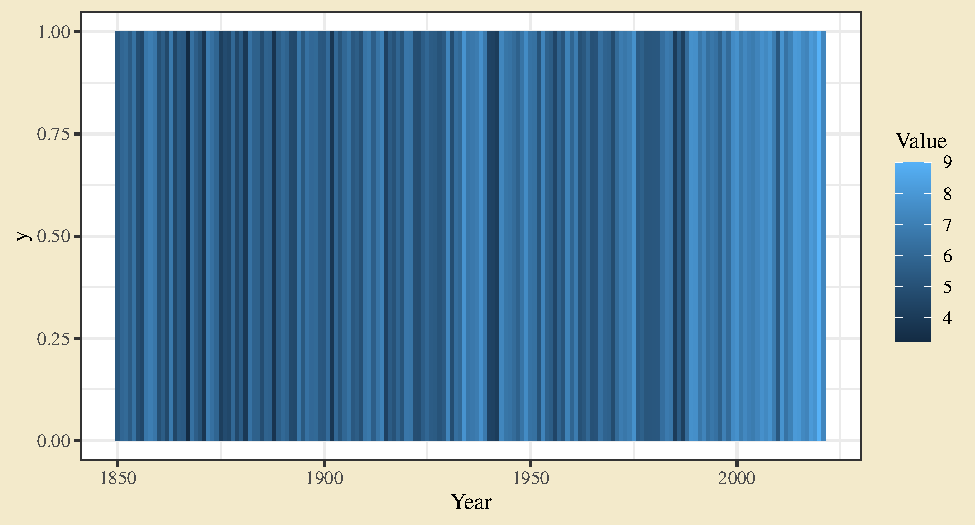
\includegraphics{R-anvisningar_files/figure-latex/unnamed-chunk-62-1} \end{center}

Ändra gärna artist på lämpligt ställe.
Vad måste läggas till för en interaktiv version av samma graf?
\end{exercise}

Hemsidan \url{https://plotly.com/r/} innehåller fler exempel för den som är intresserad.

\hypertarget{bonus-warming-stripes}{%
\section{Bonus: Warming stripes}\label{bonus-warming-stripes}}

\emph{Warming stripes} har sedan de först introducerades av Ed Hawking 2018 blivit en vanlig illustration av temperaturökning. I en warming stripe-graf anges varje år av en stapel och stapels färg ges av ett temperaturmått, vanligen årets medeltemperatur. I ggplot-terminologi har vi geometrier (staplar eller kolumner) med en x-position som ges av år och en ifylld färg som ges av temperatur.

För att göra en graf behöver vi data över temperaturer. Följande rad hämtar temperaturdata från Stockholm. Källa: \url{https://miljobarometern.stockholm.se/klimat/klimat-och-vaderstatistik/medeltemperatur/}

\begin{Shaded}
\begin{Highlighting}[]
\NormalTok{dat\_temp }\OtherTok{\textless{}{-}} \FunctionTok{read\_csv}\NormalTok{(}\StringTok{"Data/Temperatur, Stockholm.csv"}\NormalTok{)}
\end{Highlighting}
\end{Shaded}

Vi skapar nu en graf, som alltså ska ha en x-axeln given av år (\texttt{Year}) och ifylld färg som ges av temperatur (\texttt{Value}). Vi sätter höjden till 1.

\begin{Shaded}
\begin{Highlighting}[]
\FunctionTok{ggplot}\NormalTok{(dat\_temp, }\FunctionTok{aes}\NormalTok{(}\AttributeTok{x =}\NormalTok{ Year, }\AttributeTok{y =} \DecValTok{1}\NormalTok{, }\AttributeTok{fill =}\NormalTok{ Value)) }\SpecialCharTok{+}
  \FunctionTok{geom\_col}\NormalTok{()}
\end{Highlighting}
\end{Shaded}

\begin{center}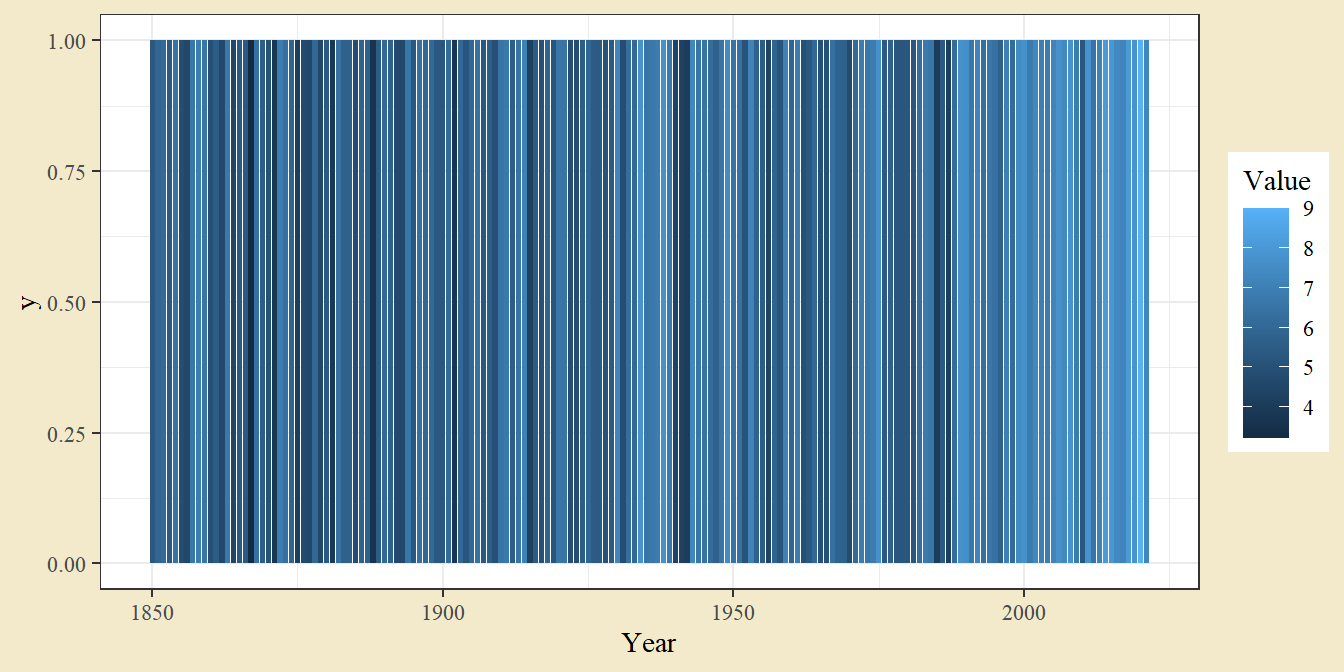
\includegraphics{R-anvisningar_files/figure-latex/unnamed-chunk-64-1} \end{center}

\begin{exercise}[Staplar utan mellanrum]
Ett första problem är att staplarna inte fyller ytan. Man kan styra staplars bredd med argumentet \texttt{width}, t.ex.

\begin{Shaded}
\begin{Highlighting}[]
\FunctionTok{ggplot}\NormalTok{(dat\_temp, }\FunctionTok{aes}\NormalTok{(}\AttributeTok{x =}\NormalTok{ Year, }\AttributeTok{y =} \DecValTok{1}\NormalTok{, }\AttributeTok{fill =}\NormalTok{ Value)) }\SpecialCharTok{+}
  \FunctionTok{geom\_col}\NormalTok{(}\AttributeTok{width =} \FloatTok{0.1}\NormalTok{)}
\end{Highlighting}
\end{Shaded}

Hitta ett värde för \texttt{width} som ger staplar utan mellanrum.
\end{exercise}

\begin{exercise}[Färgval]
Ett andra problem är att ggplots grundval för färger är från svart till blått. För klassiska warming stripes vill vi ha en skala från blått till rött. Färgerna i en skala ändras med särskilda \texttt{scale\_()}-funktioner. En färgskala för ifylld färg kan sättas med \texttt{scale\_fill\_gradientn()}, till exempel

\begin{Shaded}
\begin{Highlighting}[]
\FunctionTok{ggplot}\NormalTok{(dat\_temp, }\FunctionTok{aes}\NormalTok{(}\AttributeTok{x =}\NormalTok{ Year, }\AttributeTok{y =} \DecValTok{1}\NormalTok{, }\AttributeTok{fill =}\NormalTok{ Value)) }\SpecialCharTok{+}
  \FunctionTok{geom\_col}\NormalTok{(}\AttributeTok{width =} \FloatTok{0.1}\NormalTok{) }\SpecialCharTok{+}
  \FunctionTok{scale\_fill\_gradientn}\NormalTok{(}\AttributeTok{colours =} \FunctionTok{c}\NormalTok{(}\StringTok{"darkgreen"}\NormalTok{, }\StringTok{"blue"}\NormalTok{, }\StringTok{"white"}\NormalTok{, }\StringTok{"yellow"}\NormalTok{, }\StringTok{"purple"}\NormalTok{))}
\end{Highlighting}
\end{Shaded}

Välj färger som ger en naturlig skala från blått till rött. Funktionen \texttt{colors()} ger valbara färger i R. Några möjliga val kan vara \texttt{darkblue}, \texttt{blue}, \texttt{white}, \texttt{red}, \texttt{salmon}, \texttt{darkred}, \texttt{steelblue} och \texttt{skyblue}.
\end{exercise}

\begin{exercise}[Enkel graf]
Slutligen brukar warming stripes presenteras med så lite kringinformation som möjligt. I ggplot kan grafelement tas bort med \texttt{theme()}. Här är som exempel en graf utan y-axel, tickmärken och legend.

\begin{Shaded}
\begin{Highlighting}[]
\FunctionTok{ggplot}\NormalTok{(dat\_temp, }\FunctionTok{aes}\NormalTok{(}\AttributeTok{x =}\NormalTok{ Year, }\AttributeTok{y =} \DecValTok{1}\NormalTok{, }\AttributeTok{fill =}\NormalTok{ Value)) }\SpecialCharTok{+}
  \FunctionTok{theme}\NormalTok{(}\AttributeTok{axis.title =} \FunctionTok{element\_blank}\NormalTok{(), }
        \AttributeTok{legend.position =} \StringTok{"none"}\NormalTok{,}
        \AttributeTok{plot.background =} \FunctionTok{element\_blank}\NormalTok{(),}
        \AttributeTok{panel.background =} \FunctionTok{element\_blank}\NormalTok{(),}
        \AttributeTok{axis.text.y =} \FunctionTok{element\_blank}\NormalTok{(),}
        \AttributeTok{axis.ticks =} \FunctionTok{element\_blank}\NormalTok{())}
\end{Highlighting}
\end{Shaded}

Använd temat från exemplet för att skapa en enklare version av de warming stripes från föregående uppgift.
\end{exercise}

\hypertarget{valfria-hemuppgifter}{%
\section{Valfria hemuppgifter}\label{valfria-hemuppgifter}}

\begin{exercise}[Installera R]
Gå till \url{https://www.r-project.org/} och installera R på ditt hemma-system. Instruktioner finns i R-anvisningarnas kapitel \emph{Installation}.
\end{exercise}

\begin{exercise}[Installera RStudio]
Gå till \url{https://www.rstudio.com/} och installera RStudio på ditt hemma-system. Instruktioner finns i R-anvisningarnas kapitel \emph{Installation}.
\end{exercise}

\begin{exercise}[Öppna RStudio]
Öppna skriptet till datorövning 1 i RStudio. Notera om något ser annorlunda ut mot hur det såg ut i datorsal.
\end{exercise}

\begin{exercise}[Cheat sheets]
I början av datorövning 1 plockade vi upp en hemsida med \emph{cheat sheets} - korta instruktioner och guider till specifika R-paket. Vi kan hitta några av dem på \url{https://www.rstudio.com/resources/cheatsheets/}.
Ladda ner guiden till \texttt{ggplot2}. Hur många olika \texttt{theme\_()}-funktioner (som t.ex. \texttt{theme\_bw()}) beskrivs i guiden? Vad gör en \texttt{theme\_}-funktion?
\end{exercise}

\begin{exercise}[Timothée Chalamet]
Hitta klippet där skådespelaren Timothée Chalamet sjunger en sång om statistik. Uppskatta spårets dansbarhet och valens på en skala från noll till ett. Fundera på om det är rimligt att sätta en siffra på dansbarhet och valens.
\end{exercise}



\end{document}
